%%%%%%%%%%%%%%%%%%%%%%%%%%%%%%%%%%%%%%%%%
% Masters/Doctoral Thesis 
% LaTeX Template
% Version 2.5 (27/8/17)
%
% This template was downloaded from:
% http://www.LaTeXTemplates.com
%
% Version 2.x major modifications by:
% Vel (vel@latextemplates.com)
%
% This template is based on a template by:
% Steve Gunn (http://users.ecs.soton.ac.uk/srg/softwaretools/document/templates/)
% Sunil Patel (http://www.sunilpatel.co.uk/thesis-template/)
%
% Template license:
% CC BY-NC-SA 3.0 (http://creativecommons.org/licenses/by-nc-sa/3.0/)
%
%%%%%%%%%%%%%%%%%%%%%%%%%%%%%%%%%%%%%%%%%

%----------------------------------------------------------------------------------------
%	PACKAGES AND OTHER DOCUMENT CONFIGURATIONS
%----------------------------------------------------------------------------------------

\documentclass[
12pt, % The default document font size, options: 10pt, 11pt, 12pt
%oneside, % Two side (alternating margins) for binding by default, uncomment to switch to one side
english, % ngerman for German
singlespacing, % Single line spacing, alternatives: onehalfspacing or doublespacing
%draft, % Uncomment to enable draft mode (no pictures, no links, overfull hboxes indicated)
%nolistspacing, % If the document is onehalfspacing or doublespacing, uncomment this to set spacing in lists to single
%liststotoc, % Uncomment to add the list of figures/tables/etc to the table of contents
%toctotoc, % Uncomment to add the main table of contents to the table of contents
%parskip, % Uncomment to add space between paragraphs
%nohyperref, % Uncomment to not load the hyperref package
headsepline, % Uncomment to get a line under the header
%chapterinoneline, % Uncomment to place the chapter title next to the number on one line
%consistentlayout, % Uncomment to change the layout of the declaration, abstract and acknowledgements pages to match the default layout
]{MastersDoctoralThesis} % The class file specifying the document structure

\usepackage[utf8]{inputenc} % Required for inputting international characters
\usepackage[T1]{fontenc} % Output font encoding for international characters

\usepackage{mathpazo} % Use the Palatino font by default

%\usepackage[backend=bibtex,style=authoryear,natbib=true]{biblatex} % Use the bibtex backend with the authoryear citation style (which resembles APA)

\usepackage[style=alphabetic-verb, backend=bibtex, isbn=false, doi=false, backref=false, url=false ]{biblatex}
\addbibresource{main2.bib} % The filename of the bibliography
\usepackage[autostyle=true]{csquotes} % Required to generate language-dependent quotes in the bibliography
\usepackage{graphicx}
\usepackage{ragged2e}
\usepackage{amsmath}
\usepackage{slashbox}
\usepackage{array}
\usepackage{indentfirst}
\usepackage[]{algorithm2e}
\usepackage{algorithmic}
\usepackage{tikz}
\usepackage{pgfgantt}
\usepackage{pdflscape}
\usepackage{lscape}
\usepackage{multirow}
\newcolumntype{L}[1]{>{\raggedright\let\newline\\\arraybackslash\hspace{0pt}}m{#1}}
\newcolumntype{C}[1]{>{\centering\let\newline\\\arraybackslash\hspace{0pt}}m{#1}}
\newcolumntype{R}[1]{>{\raggedleft\let\newline\\\arraybackslash\hspace{0pt}}m{#1}}
\newcolumntype {+}{ >{\global \let \currentrowstyle \relax }}
\newcolumntype {^}{ >{\currentrowstyle }}
\newcommand {\rowstyle }[1]{\ gdef \currentrowstyle {#1} % 
  #1\ ignorespaces
}

%----------------------------------------------------------------------------------------
%	MARGIN SETTINGS
%----------------------------------------------------------------------------------------

\geometry{
	paper=a4paper, % Change to letterpaper for US letter
	inner=1.5cm, % Inner margin
	outer=3.8cm, % Outer margin
	bindingoffset=.5cm, % Binding offset
	top=1.5cm, % Top margin
	bottom=1.5cm, % Bottom margin
	%showframe, % Uncomment to show how the type block is set on the page
}

%----------------------------------------------------------------------------------------
%	THESIS INFORMATION
%----------------------------------------------------------------------------------------

\thesistitle{Thesis Title} % Your thesis title, this is used in the title and abstract, print it elsewhere with \ttitle
\supervisor{Dr. James \textsc{Smith}} % Your supervisor's name, this is used in the title page, print it elsewhere with \supname
\examiner{} % Your examiner's name, this is not currently used anywhere in the template, print it elsewhere with \examname
\degree{Doctor of Philosophy} % Your degree name, this is used in the title page and abstract, print it elsewhere with \degreename
\author{John \textsc{Smith}} % Your name, this is used in the title page and abstract, print it elsewhere with \authorname
\addresses{} % Your address, this is not currently used anywhere in the template, print it elsewhere with \addressname

\subject{Biological Sciences} % Your subject area, this is not currently used anywhere in the template, print it elsewhere with \subjectname
\keywords{} % Keywords for your thesis, this is not currently used anywhere in the template, print it elsewhere with \keywordnames
\university{\href{http://www.university.com}{University Name}} % Your university's name and URL, this is used in the title page and abstract, print it elsewhere with \univname
\department{\href{http://department.university.com}{Department or School Name}} % Your department's name and URL, this is used in the title page and abstract, print it elsewhere with \deptname
\group{\href{http://researchgroup.university.com}{Research Group Name}} % Your research group's name and URL, this is used in the title page, print it elsewhere with \groupname
\faculty{\href{http://faculty.university.com}{Faculty Name}} % Your faculty's name and URL, this is used in the title page and abstract, print it elsewhere with \facname

\AtBeginDocument{
\hypersetup{pdftitle=\ttitle} % Set the PDF's title to your title
\hypersetup{pdfauthor=\authorname} % Set the PDF's author to your name
\hypersetup{pdfkeywords=\keywordnames} % Set the PDF's keywords to your keywords
}

\begin{document}

\frontmatter % Use roman page numbering style (i, ii, iii, iv...) for the pre-content pages

\pagestyle{plain} % Default to the plain heading style until the thesis style is called for the body content

%----------------------------------------------------------------------------------------
%	TITLE PAGE
%----------------------------------------------------------------------------------------

\begin{titlepage}
\begin{center}

\vspace*{.06\textheight}
{\scshape\LARGE \univname\par}\vspace{1.5cm} % University name
\textsc{\Large Doctoral Thesis}\\[0.5cm] % Thesis type

\HRule \\[0.4cm] % Horizontal line
{\huge \bfseries \ttitle\par}\vspace{0.4cm} % Thesis title
\HRule \\[1.5cm] % Horizontal line
 
\begin{minipage}[t]{0.4\textwidth}
\begin{flushleft} \large
\emph{Author:}\\
\href{http://www.johnsmith.com}{\authorname} % Author name - remove the \href bracket to remove the link
\end{flushleft}
\end{minipage}
\begin{minipage}[t]{0.4\textwidth}
\begin{flushright} \large
\emph{Supervisor:} \\
\href{http://www.jamessmith.com}{\supname} % Supervisor name - remove the \href bracket to remove the link  
\end{flushright}
\end{minipage}\\[3cm]
 
\vfill

\large \textit{A thesis submitted in fulfillment of the requirements\\ for the degree of \degreename}\\[0.3cm] % University requirement text
\textit{in the}\\[0.4cm]
\groupname\\\deptname\\[2cm] % Research group name and department name
 
\vfill

{\large \today}\\[4cm] % Date
%\includegraphics{Logo} % University/department logo - uncomment to place it
 
\vfill
\end{center}
\end{titlepage}

%----------------------------------------------------------------------------------------
%	TITLE PAGE2
%----------------------------------------------------------------------------------------

% \begin{titlepage}
%   \begin{figure}
%     \begin{minipage}[r]{.46\linewidth}
%       \raggedright
%       
\includegraphics[scale=0.12]{Figures/upmc-logo.png}
%     \end{minipage} \hfill
%     \begin{minipage}[r]{.46\linewidth}
%       \raggedleft
%       
\includegraphics{Figures/logo-lip6.jpg}
%     \end{minipage}
%   \end{figure}
%   \large

%     \vspace*{1cm}

%     \begin{center}

%       {\bf TH\`ESE DE DOCTORAT DE \\ l'UNIVERSIT\'E PIERRE ET MARIE CURIE}

%       \vspace*{0.5cm}

%       Sp\'ecialit\'e \\ [2ex]
%       {\bf Informatique}\ \\ 

%       \vspace*{0.5cm}

%       École doctorale Informatique, Télécommunications et Électronique (Paris)

%       \vspace*{1cm}


%       Pr\'esent\'ee par \ \\


%       \vspace*{0.5cm}

      
%       {\Large {\bf Prénom NOM}}

%       \vspace*{1cm}
%       Pour obtenir le grade de \ \\[1ex]
%       {\bf DOCTEUR de l'UNIVERSIT\'E PIERRE ET MARIE CURIE} \ \\

%       \vspace*{1cm}

%     \end{center}
    
%     \flushleft{Sujet de la th\`ese :\ \\
%       \ \\
%       {\Large {\bf Le titre de ma Thèse \\ }}
      

%       \vspace*{1.5cm} 
%       \flushleft{soutenue le 30 février 2042}\\[2ex]
%       \flushleft{devant le jury composé de :  }\\[1ex]
%       \flushleft{\begin{tabular}{r@{\ }ll}
%           & M. Prénom {\sc Nom} & Directeur de thèse\\
%           & M. Prénom {\sc Nom} & Rapporteur \\
%           & M. Prénom {\sc Nom} & Rapporteur  \\
%           & M. Prénom {\sc Nom} & Examinateur  \\
%           & M. Prénom {\sc Nom} & Examinateur  \\
%         \end{tabular}
%       }
%    }
    
  
%   \end{titlepage}
%----------------------------------------------------------------------------------------
%	DECLARATION PAGE
%----------------------------------------------------------------------------------------

\begin{declaration}
\addchaptertocentry{\authorshipname} % Add the declaration to the table of contents
\noindent I, \authorname, declare that this thesis titled, \enquote{\ttitle} and the work presented in it are my own. I confirm that:

\begin{itemize} 
\item This work was done wholly or mainly while in candidature for a research degree at this University.
\item Where any part of this thesis has previously been submitted for a degree or any other qualification at this University or any other institution, this has been clearly stated.
\item Where I have consulted the published work of others, this is always clearly attributed.
\item Where I have quoted from the work of others, the source is always given. With the exception of such quotations, this thesis is entirely my own work.
\item I have acknowledged all main sources of help.
\item Where the thesis is based on work done by myself jointly with others, I have made clear exactly what was done by others and what I have contributed myself.\\
\end{itemize}
 
\noindent Signed:\\
\rule[0.5em]{25em}{0.5pt} % This prints a line for the signature
 
\noindent Date:\\
\rule[0.5em]{25em}{0.5pt} % This prints a line to write the date
\end{declaration}

\cleardoublepage

%----------------------------------------------------------------------------------------
%	QUOTATION PAGE
%----------------------------------------------------------------------------------------

\vspace*{0.2\textheight}

\noindent\enquote{\itshape Thanks to my solid academic training, today I can write hundreds of words on virtually any topic without possessing a shred of information, which is how I got a good job in journalism.}\bigbreak

\hfill Dave Barry

%----------------------------------------------------------------------------------------
%	ABSTRACT PAGE
%----------------------------------------------------------------------------------------

\begin{abstract}
\addchaptertocentry{\abstractname} % Add the abstract to the table of contents
The Thesis Abstract is written here (and usually kept to just this page). The page is kept centered vertically so can expand into the blank space above the title too\ldots
\end{abstract}

%----------------------------------------------------------------------------------------
%	ACKNOWLEDGEMENTS
%----------------------------------------------------------------------------------------

\begin{acknowledgements}
\addchaptertocentry{\acknowledgementname} % Add the acknowledgements to the table of contents
The acknowledgments and the people to thank go here, don't forget to include your project advisor\ldots
\end{acknowledgements}

%----------------------------------------------------------------------------------------
%	LIST OF CONTENTS/FIGURES/TABLES PAGES
%----------------------------------------------------------------------------------------

\tableofcontents % Prints the main table of contents

\listoffigures % Prints the list of figures

\listoftables % Prints the list of tables

%----------------------------------------------------------------------------------------
%	ABBREVIATIONS
%----------------------------------------------------------------------------------------

\begin{abbreviations}{ll} % Include a list of abbreviations (a table of two columns)

\textbf{LAH} & \textbf{L}ist \textbf{A}bbreviations \textbf{H}ere\\
\textbf{WSF} & \textbf{W}hat (it) \textbf{S}tands \textbf{F}or\\

\end{abbreviations}

%----------------------------------------------------------------------------------------
%	PHYSICAL CONSTANTS/OTHER DEFINITIONS
%----------------------------------------------------------------------------------------

\begin{constants}{lr@{${}={}$}l} % The list of physical constants is a three column table

% The \SI{}{} command is provided by the siunitx package, see its documentation for instructions on how to use it

Speed of Light & $c_{0}$ & \SI{2.99792458e8}{\meter\per\second} (exact)\\
%Constant Name & $Symbol$ & $Constant Value$ with units\\

\end{constants}

%----------------------------------------------------------------------------------------
%	SYMBOLS
%----------------------------------------------------------------------------------------

\begin{symbols}{lll} % Include a list of Symbols (a three column table)

$a$ & distance & \si{\meter} \\
$P$ & power & \si{\watt} (\si{\joule\per\second}) \\
%Symbol & Name & Unit \\

\addlinespace % Gap to separate the Roman symbols from the Greek

$\omega$ & angular frequency & \si{\radian} \\

\end{symbols}

%----------------------------------------------------------------------------------------
%	DEDICATION
%----------------------------------------------------------------------------------------

\dedicatory{For/Dedicated to/To my\ldots} 

%----------------------------------------------------------------------------------------
%	THESIS CONTENT - CHAPTERS
%----------------------------------------------------------------------------------------

\mainmatter % Begin numeric (1,2,3...) page numbering

\pagestyle{thesis} % Return the page headers back to the "thesis" style

% Include the chapters of the thesis as separate files from the Chapters folder
% Uncomment the lines as you write the chapters

\sloppy
\chapter{Placement}
\label{chap:Placement}

\section{Introduction}
\label{sec:Placement-Introduction}
Les systèmes-sur-puce modernes contiennent tant des circuits numériques que des circuits analogiques. La conception de circuits numériques a été particulièrement automatisée par des outils de conception assistée par ordinateur tandis que la conception de circuits analogiques est restée manuelle. Avec l'évolution des nouvelles technologies nanométriques, cela implique un travail manuel long et sujet à l'erreur humaine. \newline 

\indent Dans le cadre des circuits analogiques, les parasites du dessin des masques et les contraintes de procédés de fabrication augmentent drastiquement la complexité de la tâche quant au placement des modules du circuit. Il devient essentiel d'introduire des outils de placement dédiés aux circuits analogiques dans le but d'accélérer aussi bien le cycle de conception que l'effort de conception. \newline 

\indent La phase de placement pour les circuits mixtes et analogiques a une influence importante sur les performance du circuit. La relation de placement entre l'ensemble des modules, et plus particulièrement celle entre les modules appariés, est importante afin de préserver au plus possible l'environnement adéquate de fonctionnement des modules en tenant compte des parasites engendrés par le dessin des masques. \newline

\indent Dans ce chapitre, nous discuterons de l'étude du problème du placement des circuits mixtes et analogiques. \newline

\indent Dans la section \ref{sec:Placement-SoA-topologie}, nous énumérons les principales représentations topologiques du plan de masse de l'état de l'art. Ces représentations utilisent des graphe traduisant des relations de placement entre l'ensemble des modules d'un circuit. Leur spécificité avec leurs avantages et inconvénients et les contraintes qu'elles sont capables de prendre en compte dans le choix d'un placement optimal seront explicités. \newline 

\indent Dans la section \ref{sec:Placement-SoA-optimization}, nous exposerons la phase d'optimisation que la majorité de l'état de l'art utilise dans le cadre de la recherche d'une solution de placement optimale. Les algorithmes de recuit simulé ont souvent opté pour leur capacité à produire de bons résultats en temps suffisamment court. Ces algorithmes sont également relativement simples à implémenter et peuvent être facilement enrichis pour des conditions supplémentaires. \newline

\indent Dans la section \ref{sec:Placement-Implémentation}, nous présenterons notre approche du problème du placement des circuits mixtes et analogiques. Notre représentation topologique ainsi que notre méthodologie d'optimisation y sera détaillées. Cette section contiendra une partie de notre structure de données utilisée tout au long de la génération du placement routage. \newline

\indent Dans la section \ref{sec:Placement-Exemple}, les détails de la méthodologie de placement seront illustrés par un exemple contenant des contraintes de placement répandues. Les interventions du concepteur seront énumérés avec clarté dans le but de mettre en avant son rôle dans le choix de la solution de placement.

\section{\'Etat de l'art des algorithmes de placement}
\label{sec:Placement-SoA}

\indent Le problème de placement abordé par les outils de CAO dédiés aux dessins des masques numériques et analogiques consistent à explorer un grand espace de solutions de configurations de placement faisables et non faisables en utilisant une représentation du plan de masse couplée à une optimisation stochastique telle que l'algorithme de recuit simulé. A la différence des circuits numériques, les circuits analogiques doivent prendre en considération des contraintes de placement supplémentaires liées aux parasites du dessin des masques. L'état de l'art des approches de placement pour circuits mixtes et analogiques sera abordé dans les sections suivantes. 
\subsection{Les représentations topologiques de plan de masse}
\label{sec:Placement-SoA-topologie}

Afin de pouvoir générer un placement légal respectant plusieurs contraintes de placement analogiques, la majorité des études récentes emploie une représentation sous forme de graphe. On distigune deux catégories de représentations: les représentations absolues et les représentations topologiques. Les représentations absolues \cite{Jepsen83} sont principalement dans les anciennes méthodes de placement et consiste à associer à chacun des modules du circuit une coordonnée par rapport à un point de référence. Cette représentation permet la superposition illégale de modules lors de la phase d'optimisation dû au fait qu'il n'existe pas de relation de placement entre les modules. Cette approche doit alors être en mesure explorer un très grand espace de solutions comprenant tant des placements faisables que non faisables. Cela se traduit par des temps d'exécution long causés par le grand nombre de mouvements nécessaires pour obtenir un dessin des masques satisfaisant. Il est également possible qu'en plus du long temps d'exécution, il ne garantie pas toujours de solutions faisables. L'ajustement de la fonction de coût pour éviter les recouvrements de modules peut requérir un effort conséquent. \newline

En opposition aux représentations absolues, les représentations topologiques ne font pas face à des problèmes de recouvrements, elles consistent à définir des relations de positions entre les modules d'un circuit. Ces représentations sont largement utilisés pour des raisons d'efficacité et de flexibilités à pouvoir satisfaire des contraintes pour un moindre coût en termes de nombre de mouvements comparées aux représentations absolues. On présentera dans les sous-sections suivantes les représentations topologiques les plus utilisées de l'état de l'art. 
\subsubsection{Les slicing models}
Les {\it slicing models} \cite{Wong1986} font parties des premières représentations topologiques utilisées. Ces {\it slicing models} sont représentés à l'aide d'un graphe appelé {\it slicing tree}. Un {\it slicing tree} est un arbre dans lequel chaque noeud interne peut être obtenu par découpes récursives du circuit (Fig. \ref{fig:1}). A partir de la région totale du circuit représentant la racine de l'arbre, le circuit sera découpé de manière hiérarchique, alternativement de manière horizontal et vertical, jusqu'à atteindre les feuilles de l'arbre représentant les modules du circuit ou bien des espaces de routage. L'ensemble des rectangles terminaux dû aux découpes sera toujours représenté par une feuille. \newline
\begin{figure}[h]
\begin{center}
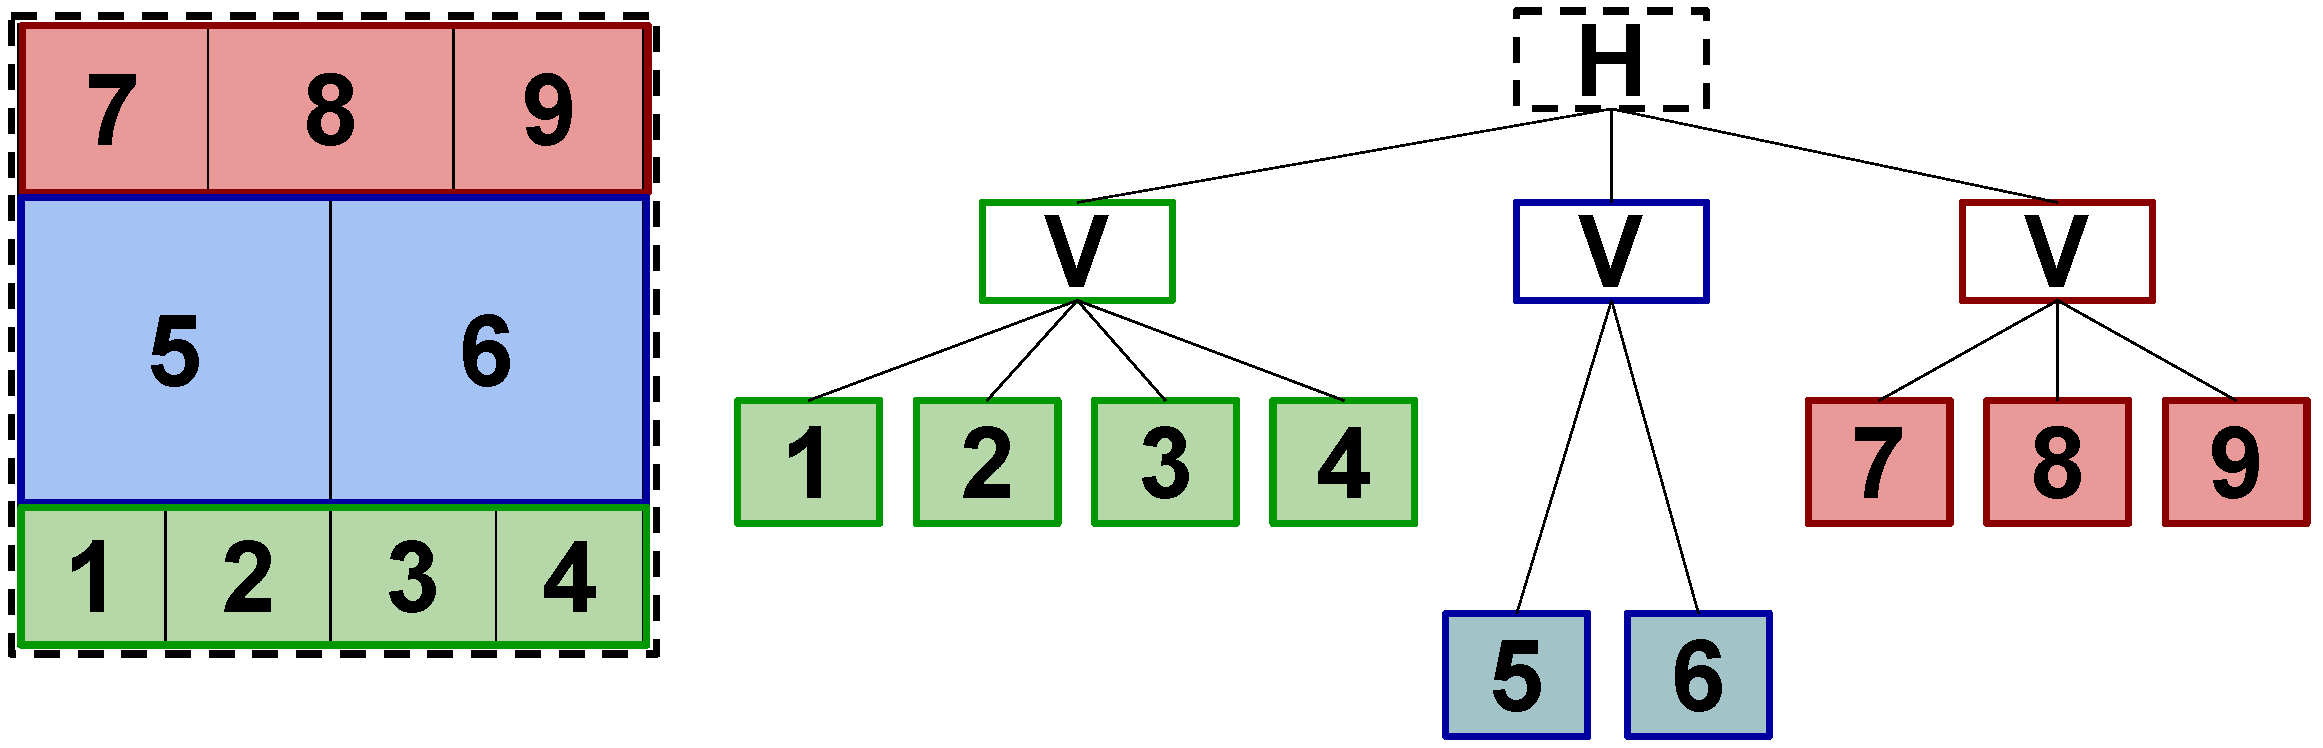
\includegraphics[height=0.17\textheight]{Figures/1.pdf}
\caption{Exemple de placement et sa représentation en {\it slicing tree} ou "H" définit une coupe horizontal et "V" une coupe vertical.} 
\label{fig:1}
\end{center}
\end{figure}  \newline
\cite{Abthoff1996} concentre son optimisation sur la surface totale du circuit ainsi que la longueur total des {\it nets} dont l'amélioration est 5 fois plus courte comparé à la non prise en considération. L'optimisation prend en compte les contraintes de proximité, de modules pré-placés et de symmetries. \cite{Prieto1997} considère les parasites d'interconnection dans la phase d'optimisation avec une prise en compte simultanée du placement et routage. Ils sont en mesure de maintenir des symmetries de groupes de modules. \cite{Young1998} étend l'approche de \cite{Wong1986} afin de pouvoir considérer des modules pré-placés, de contraintes de bordure \cite{Young1999} et de proximité \cite{Young2000}. \cite{lina2012} améliore la formulation des {\it slicing trees} en introduisant des conditions de symmétries pour des groupes de modules. \cite{Wu2012} introduit la prise en compte des contraintes de sens du courant dans les structures en {\it slicing tree} en plus des symétries. \newline

Puisque tous les circuits n'ont pas une structure en tranche, le désavantage de cette topologie est que la densité de la solution de placement peut être dégradé ce qui peut être notable lorsque les modules d'un circuit ont des rapports hauteur/largeur très hétérogènes. De plus, la structure des {\it slicing trees} ne permet pas de représenter toutes les placement possibles (Fig. \ref{fig:2}). Suite à ces limitations, des représentations avec des structures {\it non-slicing} se sont succédé. Les {\it sequence pairs}, les {\it B*-trees}, les {\it Ordered-Trees - O-tree} et les {\it Transitive Closure Graphs - TCG} seront présentés dans les sous-sections suivantes.
\begin{figure}[h]
\begin{center}
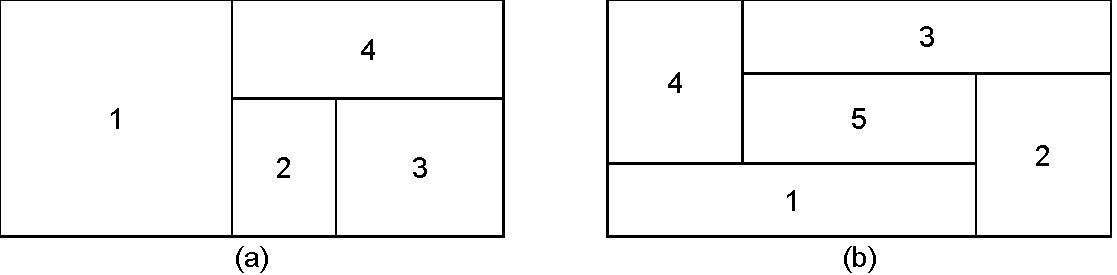
\includegraphics[height=0.15\textheight]{Figures/2.pdf}
\caption{Exemple d'un placement représentable par un {\it slicing tree} (a) et d'un placement non représentable (b)} 
\label{fig:2}
\end{center}
\end{figure}
\subsubsection{Les sequence pair}
Les {\it sequence pairs} sont utilisés dans le context des placements de circuits analogiques pour la première fois par \cite{Balasa2000}. Une {\it sequence pair} donnée pour ensemble de modules est une paire de séquences contenant l'ensemble des modules. Par example, $(abc, cba)$ est une {\it sequence pair} pour l'ensemble de module \{$a,b,c$\}. Pour un placement donné, la sequence pair correspondante est obtenue par la construction des échelons positifs et négatifs de chacun des modules (Fig. \ref{fig:3}). L'échelon positif (négatif) d'un module contient 3 parties: l'échelon haut-droit (gauche-haut), l'échelon bas-gauche (droite-bas) et la ligne diagonale effectuant la connexion. L'échelon  haut-droite (bas-gauche, gauche-haut, droite-bas respectivement) d'un module est $A$ est dessiné en suivant les règles suivantes:

\begin{enumerate}
\item On part de coin supérieur droit (inférieur gauche, supérieur gauche et inférieur droit respectivement) du module $A$.
\item On change la direction alternativement haut (bas, gauche et droite respectivement) et droit (gauche, haut et bas respectivement) jusqu'à atteindre le coin supérieur droit (inférieur gauche, supérieur gauche et inférieur droit respectivement) du placement sans croiser:
\begin{itemize}
\item Les bordures des autres modules
\item Les lignes précédemment tracées
\end{itemize}
\end{enumerate}
En utilisant l'ordre des séquences des échelons positifs et négatifs (de la gauche vers la droite), une paire ordonnée, ($\Gamma_+, \Gamma_-$), de séquences de modules peut être placé. La Fig. \ref{fig:3} montre le placement résultant de ses échelons négatifs et positifs avec de ses séquences respectives. A partir d'une {\it sequence pair}, il est également possible d'en dégager les contraintes géométriques (horizontal ou vertical) entre deux modules.

\begin{figure}[h]
\begin{center}
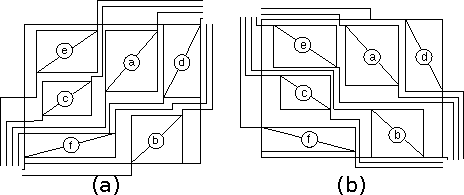
\includegraphics[height=0.22\textheight]{Figures/3.pdf}
\caption{(a) \'Echelons positifs résultant et $\Gamma_+=ecadfb$. (b) \'Echelons négatifs résultant et $\Gamma_-=fcbead$.} 
\label{fig:3}
\end{center}
\end{figure}

H. Murata et al. \cite{Murata1996} sont les premiers à introduire le concept de {\it sequence pair} pour des applications de dessins des masques {\it VLSI} durant une période pendant laquelle les {\it slicing models} étaient populaires mais ne produisaient pas des résultats assez satisfaisant. \cite{Balasa2000} adresse l'utilisation des {\it sequence pairs} dans le cadre du placement pour circuits analogiques avec une prise en compte de contraintes de symmétries et \cite{Balasa2001} améliore leur temps de calcul par la suite. \cite{Cheong2006} ajoute la considération d'alignement et de contraintes de proximités des modules en plus des symmétries. \cite{Long2006} oriente leur attention sur du placement vis à vis du sens du courant tout en tenant compte des symétries. \cite{Nakatake2010} porte leur attention sur les contraintes de regularités couplés aux contraintes de symmétries. \cite{Xiao10} prends en considération des contraintes de congestions pour le routage en évaluant la congestion des placements donnés. 

\subsubsection{Les O-trees}
\begin{figure}[h]
\begin{center}
  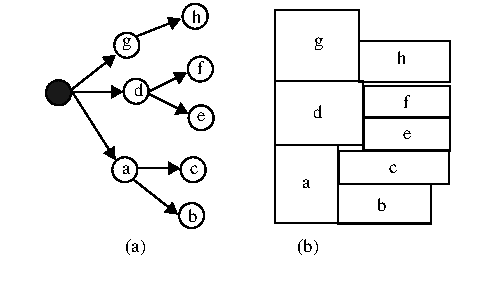
\includegraphics[height=0.24\textheight]{Figures/5.pdf}
  \caption{(a) Une représentation en {\it O-tree} et (b) son placement correspondant.}
\label{fig:5}
\end{center}
\end{figure}
Un ({\it Ordered Tree (O-tree)}) étend le principe des {\it B*-tree}  à une représentation du plan de masse de type {\it non-slicing} avec une complexité inférieur à celle des {\it slicing models}. \'Etant donné un placement de $n$ modules, un {\it O-tree} correspondant possède $n+1$ noeuds encodé par ($T,\pi$), o\`u $T$ correspond à une chaine de caractères de 2$n$-bit identifiant la structure de l'arbre et $\pi$ représente l'ordre des noms des modules sans considérer la racine de l'arbre. Lorsqu'on parcourt l'arbre en profondeur, "0" correspondant à une arête descendante, et "1" à une arête ascendante. Cette méthode permet de réduire les redondances et le temps d'exécution est plus rapide que celui des représentations en {\it sequence pair}. \newline

Cette méthodologie est introduite par \cite{Guo1999}, \cite{FlorinBalasa2000} et \cite{LinfuXiao2009} élargies les types contraintes de symétries considérées.

\subsubsection{Les B*-trees et HB*-trees}
\begin{figure}[h]
\begin{center}
  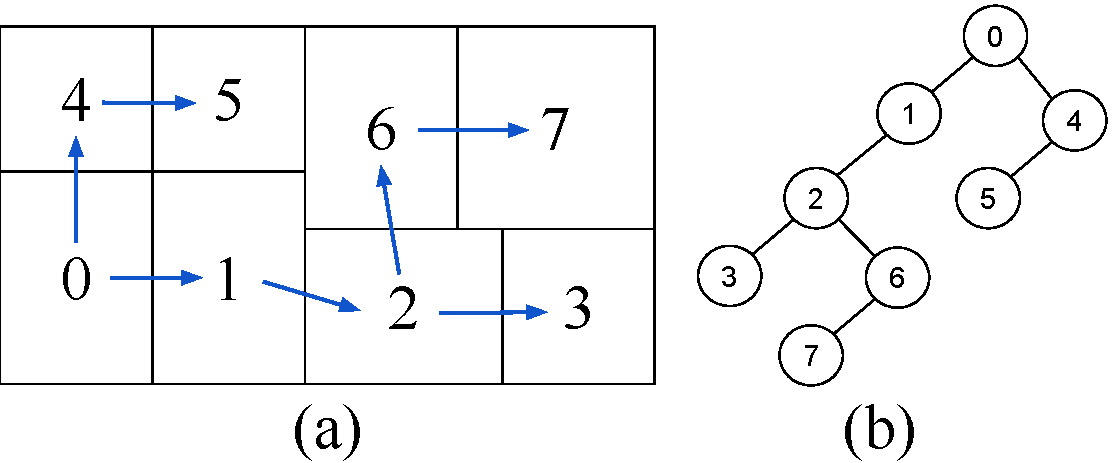
\includegraphics[height=0.19\textheight]{Figures/4a.pdf}
  \caption{(a) Placement compact. (b) Représentation en {\it B*-tree} du placement compact (a).}
\label{fig:4a}
\end{center}
\end{figure}
 Les ({\it Ordered Binary Trees - B*-trees}) sont des arbres couramment utilisés pour représenter un placement compacte de modules dans lequel tous les modules ne peuvent plus se déplacer vers la gauche et vers le bas. Chaque module d'un circuit est représenté par un noeud dans un {\it B*-tree}. La racine d'un {\it B*-tree} correspond au module situé dans le coin inférieur gauche, il s'agit du module 0 sur la Fig. \ref{fig:4a}. Le noeud de gauche du module 0 représente le module de droite et adjacent au module 0, il s'agit du module 1. Le noeud de droite du module 1 représente le module au dessus et adjacent au module 0, il s'agit du module 4. La Fig. \ref{fig:4a} montre un placement et sa représentation en {\it B*-tree} correspondante. \newline

Les {\it B*-trees} sont introduits par \cite{Balasa2000.2} et \cite{Chang2000} dans le but d'utiliser une réprésentation succédant aux {\it O-trees}. Cette approche est amélioré en incorporant les contraintes de symmétrie par \cite{Balasa2002} dans le cadre des circuits analogiques. \cite{Maruvada2005} améliore le temps d'execution de 20\% à 30\%. \cite{Strasser08} propose une approche déterministe permettant une meilleure reproductabilité du placement. \newline

La représentation des B* avec s'enrichie avec l'utilisation des {\it Hierarchical Ordered Binary Trees - HB*-trees} \cite{Lin09} dans le but d'ajouter des contraintes hierarchies et groupes de symétries. \cite{Lin2010} y ajoute la prise en compte de contraintes de bordure. Cette représentation est ensuite utilisé pour différentes contraintes d'optimisation, telle que pour des contraintes de température \cite{Lin11} ou de régularité \cite{Chou2011} et avec de meilleur optimisation de temps d'execution \cite{Tsao2011}.

\subsubsection{Les Transitive Closure Graph}
Les {\it Transitive Closure Graphs (TCG)} décrivent les relations géométriques entre les modules d'un circuit en se basant sur deux graphes: un {\it Horizontal transitive closure graph $G_h$} et un {\it Vertical transitive closure graph $G_v$}. Dans le {\it $G_h$} (respectivement {\it $G_v$}), une arête $<v_i,v_j>$ exprimé que le module $m_i$ se trouve à gauche de (respectivement en bas de) la cellule $m_j$. Le poid associé à l'arête dans {\it $G_h$} (respectivement {\it $G_v$}) correspond à la largeur (respectivement hauteur) du module associé. La Fig. \ref{fig:6} montre un example de placement avec sa représentation {\it TCG}. \newline

\begin{figure}[h]
\begin{center}
  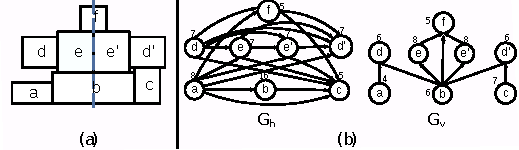
\includegraphics[height=0.17\textheight]{Figures/6.pdf}
  \caption{(a) Placement compact. (b) Représentation en {\it TCG} du placement compact (a).}
\label{fig:6}
\end{center}
\end{figure}

Les {\it Transitive Closure Graphs (TCG)} sont introduits par \cite{Lin2001} dans le contexte d'opter pour des solutions différentes des {\it sequence pairs} et des {\it B*-trees}. \cite{Zhang2008} y ajoute la considération des contraintes de symmétrie. Les {\it Transitive Closure Graphs TCG)} sont étendus au {\it TCG-S} par \cite{Lin2004a} et \cite{Ming2005} avec lesquels la phase de compactage est plus performante est inspiré de celle des {\it sequence pairs}.

\subsubsection{Sommaires des contraintes des représentations}
Au cours de ces deux dernières décennies, de nombreuses représentations topologiques ont été utilisées en couplage avec diverses contraintes. L'ensemble des articles mentionnés précédemment sont rassemblés dans le tableau récapitulatif \ref{tab:constraints}. A partir d'une représentation du plan de masse considérant les contraintes du concepteur, il en vient ensuite la phase d'optimisation du placement. Elle consiste à explorer l'espace des solutions de placement afin de trouver une solution en un temps raisonnable.
\begin{table}[h]
\footnotesize
\centering
\caption{Tableau récapitulatif de l'état de l'art des représentations de placement pour les circuits analogiques }
\label{tab:constraints}
  \begin{tabular}{|L{100pt}|C{50pt}|C{50pt}|C{50pt}|C{50pt}|C{50pt}|}
    \hline
    Contraintes                              & Slicing-tree                                                         & Sequence Pair & O-tree & B*-tree et HB*-tree & TCG \\ \hline
    Symmétries                                & \cite{Abthoff1996}, \cite{Prieto1997}, \cite{lina2012}, \cite{Wu2012}& \cite{Balasa2000}, \cite{Balasa2001}, \cite{Cheong2006}, \cite{Nakatake2010}, \cite{Xiao10}& \cite{FlorinBalasa2000}, \cite{LinfuXiao2009}& \cite{Balasa2000.2}, \cite{Balasa2002}, \cite{Maruvada2005}, \cite{Strasser08}, \cite{Lin09}, \cite{Lin2010}, \cite{Lin11}, \cite{Chou2011}, \cite{Tsao2011} &  \cite{Zhang2008}, \cite{Ming2005}   \\ \hline
    Symétrie de groupes                       & \cite{Wu2012}                                                        & \cite{Xiao10} & & \cite{Lin09}, \cite{Lin2010}, \cite{Lin11} &     \\ \hline
    Centrage géométrique                      &                                                                      & \cite{Xiao10} & \cite{LinfuXiao2009}& \cite{Strasser08}                    &     \\ \hline
    Sens du courant                           & \cite{Wu2012}                                                        & \cite{Long2006}&        &                    &     \\ \hline
    Température                               &                                                                      &                &        & \cite{Lin11}       &     \\ \hline
    Régularité                                &                                                                      &\cite{Nakatake2010}&        &  \cite{Chou2011}&     \\ \hline
    Proximité                                 & \cite{Abthoff1996}, \cite{Young2000}                                 &\cite{Cheong2006}&        & \cite{Strasser08} &     \\ \hline
    Régularité                                &                                                                      &               &        & \cite{Balasa2000.2} &     \\ \hline
    Modules pré-placés                        & \cite{Abthoff1996}, \cite{Young1998}                                 &               &        & \cite{Tsao2011}     &     \\ \hline
    Bordures                                  & \cite{Young1999}                                                     &               &        & \cite{Lin2010}, \cite{Tsao2011}      &     \\ \hline
    Routage                                   & \cite{Prieto1997}                                                    &\cite{Xiao10}  &        &                     &     \\ \hline
  \end{tabular}
\end{table} \newpage

\subsection{Les méthodes d'optimisation de placement}
\label{sec:Placement-SoA-optimization}
La majeure partie des approches de l'état de l'art utilise une représentation topologique parmi celles mentionnées dans la section précédente, avec laquelle on applique la méthode du recuit simulé. Cette méthode introduite par \cite{kirkpatrick83} est une technique probabiliste d'approximation de l'optimum global d'une fonction donnée. C'est à dire qu'il s'agit d'une métaheuristique permettant d'estimer l'optimisation globale dans un grand espace de recherche. Le principe s'inspire du processus de recuit des métaux en métallurgie dans lequel le refroidissement d'un matériau est contrôlé. Cela se traduit par une probabilité d'acceptation dégressive des mauvaises solutions dans l'espace de solutions exploré. \newline

Le fonctionnement de l'algorithme du recuit simulé se déroule par les étapes suivantes:
\begin{enumerate}
\item \label{enum:i1} L'algorithme sélectionne une transformation aléatoire prédéfinie sur la solution courante 
\item \label{enum:i2} On mesure la qualité de la solution sélectionnée 
\item On sauvegarde la nouvelle solution ou bien on décide maintenir la solution courante en se basant sur une probabilité dépendant de la qualité précédemment évaluée
\item Le paramètre de température diminue se traduisant par une augmentation de la probabilité du choix de la meilleure solution et une diminution de la probabilité du choix de mauvaise qualité
\end{enumerate}
Le tirage au sort (étape \ref{enum:i1}) des transformations est déterminé en fonction de l'approche choisie. Ces transformations dépendent de la représentation utilisée, une transformation revient à perturber le graphe représentant le placement de la solution courante. Il peut s'agir d'une rotation d'un module ou d'un échange de position entre deux modules. \newline 

La spécification des contraintes de placement d'un concepteur se définit par la formulation d'une fonction de coût qui nous permet d'évaluer la qualité (étape \ref{enum:i2}) de la solution sélectionnée . Afin d'illustrer le fonctionnement général d'une fonction de coût, considérons une optimisation sur une contrainte de surface global et d'une longueur de fil, la fonction de coût se présenterait de la façon suivante:
\begin{equation}\label{eq:1}
  Cost(F) =  \alpha . A_{normalis \acute{e}} + \beta . W_{normalis \acute{e}}
\end{equation}
avec $\alpha$ et $\beta$ étant des paramètres de réglages permettant d'influencer l'importance de la contrainte considérée, $A_{normalis \acute{e}}$ représentant la surface total occupée normalisée et $W_{normalis \acute{e}}$ la longueur de fil totale normalisée.
\newpage
\section{Implémentation}
\label{sec:Placement-Implémentation}
Parmi l'ensemble des méthodologies de placement analogique, la majorité d'entre elle présente une capacité à produire un placement tenant compte d'une ou plusieurs contraintes du concepteur. L'utilisation de métaheuristique permet de produire des résultats optimisés pour les contraintes considées dans la fonction de coût. Néanmoins, la complexité des contraintes des circuits analogiques et mixtes peuvent rendre difficile l'ajustement des paramètres de la fonction de coût. Dans la section suivante, nous présenterons l'approche pour laquelle nous avons opté ainsi que les raisons qui nous ont poussés à faire ces choix. Un exemple illustrera notre méthodologie et notre outil de placement.

\subsection{Notre approche de placement}
La phase de placement est une étape complexe dans la réalisation d'un circuit tant pour les circuits numériques qu'analogiques mais se différencie par leur problème. Dans le cadre des circuits numériques, le problème consiste à placer un grand nombre de cellules tout en minimisant la surface occupée et la longueur de fils des interconnections. En règle générale, la phase de placement est découplé de la phase de routage. Quant au problème de placement des circuits analogiques, il consite à placer un plus faible nombre de cellules tout en respectant les deux contraintes mentionnées précédemment, mais également une multitude de contraintes simultanément pouvant provenir de plusieurs domaines (électrique, mécanique ou bien thermique). \newline

Ces considérations ont amenées à la création de représentations topologiques et méthodes d'optimisation mentionnée dans les sous-sections \ref{sec:Placement-SoA-topologie} et \ref{sec:Placement-SoA-optimization}. En étudiant l'état de l'art du placement analogique, nous pensons que certains aspects nécessite une particulière attention ainsi que les limites d'une grande majorité des approches. Ce sont en tenant compte des considérations suivantes que nous avons effectué des choix dans le cadre de notre approche de placement:

\begin{itemize}
\item \textbf{Interventions du concepteur:} La conception du dessin des masques dans le domaine numérique est une étape particulièrement automatisé par rapport au domaine analogique. Du fait de la complexité du jeu de contraintes à gérer, nous jugeons qu'il est préférable de ne pas rendre l'automatisation du placement et du routage aussi automatique que dans le domaine numérique. Le placement d'un circuit dépend de plusieurs facteurs. L'environnement dans lequel va fonctionner le circuit comprend la prise en compte des effets des procédés de fabrication et des leurs effets parasites. Le facteur qui nous parait particulièrement important est que l'expérience d'un concepteur peut énormément influencer les choix de placement dans la gestion des compensations des effets parasites. Sans la prise en compte de cette experience, les outils de placement pour circuits analogiques produiront la plupart du temps des résultats insatisfaisant. Il en vient qu'il est nécessaire que le concepteur ait la possibilité des d'effectuer des interventions significatives. Notre approche s'oriente vers une approche o\`u l'automatisation est moindre en comparaison à l'état de l'art mais l'influence du concepteur sur le résultat final d'avantage prise en compte.

\item \textbf{Gestion des contraintes:} On observe dans l'état de l'art qu'une grande diversité de contraintes pour chaque représentation topologique en particulier pour les {\it B*-trees}. On remarque que la gestion des contraintes est relativement automatisé, il n'est pas toujours évident de connaître la capacité des paramètres à être modifier. L'ajustement de ces paramètres est généralement fixé suite à de nombreux essaies et ne peut être l'unique manoeuvre de jeu du concepteur. Dans notre méthodologie de placement, les contraintes gérées de manière automatique sont uniquement les contraintes de symétries. Nous utilisons une approche en {\it slicing tree}, cette représentation sera défini par le concepteur. Définir le {\it slicing tree} revient à laisser le choix aux concepteurs de juger l'importance de chacune des contraintes nécessaires à être prise en compte.

\item \textbf{Ajustabilité du placeur:} Le recuit simulé associé à une des représentations de l'état de l'art permet de générer des placements suivant en certains nombres de critères. Malgrés la qualité des placements produits, il est souvent nécessaire de réaliser des modifications diverses. Il peut s'agir de modification de placement entre deux blocks ou bien un simple repositionnement de certains modules. Dans la mesure o\`u les concepteurs souhaitent réaliser ce type de modifications, il peut s'avérer difficile de réajuster la représentation topologique ou bien encore la position de l'ensemble du circuit pour des raisons de compactions. Dans le cadre du {\it slicing tree}, le repositionnement ou bien le changement de taille d'un module est facile de part la structure du plan de masse en découpe. Tout comme mentioné dans le point précédent, la définition du {\it slicing tree} est une tâche réalisée par le concepteur, lui permettant d'avoir un contrôle important sur le placement relatif des modules.

\item \textbf{Placement déterministe:} Les algorithmes d'optimisation ne permettent pas toujours de générer des placements prévisibles. Certains d'entre eux permettent une certaine reproductibilité à maintenant les jeux de paramètres du recuit simulé en tenant compte de la température de départ et de la fonction de refroidissement. Néanmoins, les aspects aléatoires des probabilités des choix de placement peuvent rendre l'algorithme non déterministe. Le non-déterminisme rend l'évaluation des paramètres d'entrées difficiles ainsi que l'ajustabilité du placeur. L'approche que nous avons adopté permet un calcul des placements valides de manière déterministe. Nous jugeons que cette caractéristique est particulièrement utile dans les phases de débug.
\begin{figure}[h]
\begin{center}
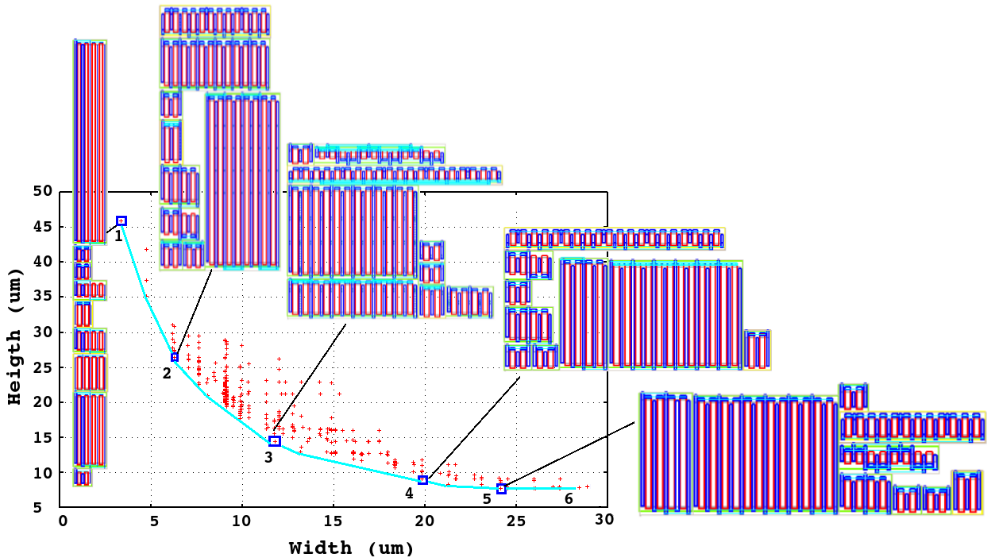
\includegraphics[height=0.25\textheight]{Figures/7-1.png}
\caption{Notre approche permet la génération rapide de plusieurs placements}
\label{fig:3}
\end{center}
\end{figure}
\item \textbf{Choix multiple de placements:} Le recuit simulé permet de générer un unique placement optimisé respectant au mieux les contraintes données considérées en entrée. Pour les même raisons mentionées dans les points précédents, cet unique placement sera probablement rarement choisi par tous les concepteurs. Nous pensons qu'il est nécessaire d'avoir la capacité à générer plusieurs placements afin que les concepteurs puissent choisir une solution qui lui conviennent. Certains placements peu compactes pourraient être des résultats de placements plus satisfaisant aux yeux des concepteurs dans certaines situations. Les placements identifiés par notre outil de placement sont disposés sur un graphe o\`u chaque placement est représenté par un point défini par la largeur et hauteur du placement global.

\item \textbf{Placement déterministe:} Les algorithmes d'optimisation ne permettent pas toujours de générer des placements prévisibles. Certains d'entre eux permettent une certaine reproductibilité à maintenant les jeux de paramètres du recuit simulé en tenant compte de la température de départ et de la fonction de refroidissement. Néanmoins, les aspects aléatoires des probabilités des choix de placement peuvent rendre l'algorithme non déterministe. Le non-déterminisme rend l'évaluation des paramètres d'entrées difficiles ainsi que l'ajustabilité du placeur. L'approche que nous avons adopté permet un calcul des placements valides de manière déterministe. Nous jugeons que cette caractéristique est particulièrement utile dans les phases de débug.


\begin{table}[h]
\footnotesize
\centering
\caption{Comparison of area usage and runtime for different approaches on 1-S symmetry placement  \cite{Xiao10}}
\label{tab:implémentation}
\begin{tabular}{|c|c|c|c|c|c|c|c|c|c|c|}
\hline
\multirow{2}{*}{Data Set} & \multirow{2}{*}{\begin{tabular}[c]{@{}c@{}}Block \\ No.\end{tabular}} & \multirow{2}{*}{\begin{tabular}[c]{@{}c@{}}1-D\\ Groups\end{tabular}} & \multicolumn{2}{c|}{Sequence Pair} & \multicolumn{2}{c|}{Slicing Tree} & \multicolumn{2}{c|}{HB*-tree} & \multicolumn{2}{c|}{B*-tree} \\ \cline{4-11} 
                          &                                                                       &                                                                       & Area        & Time      & Area        & Time      & Area           & Time         & Area          & Time         \\ \hline
Bench 1                   & 65                                                                    & 8,12,5                                                                & 114.9       & 780       & 114.9       & 246       & 104.7          & 22           & 104.9         & 337          \\ \hline
Bench 2                   & 110                                                                   & 16,6,6,12,4                                                           & 110.4       & 2824      & 109.4       & 726       & 105.7          & 43           & 107.7         & 387          \\ \hline
\end{tabular}
\end{table}

\item \textbf{Temps d'exécution faible:} Les contraintes de placement pour les circuits analogiques ainsi que le nombre inférieur de cellules réduit fortement l'espace de solutions en comparaison avec le problème du placement des circuits numériques. Le temps d'execution du recuit simulé nécessite un certain temps quelque ce soit le type de topologie employé \cite{Xiao10}. La génération de multiple placements de notre approche nécessite des temps de placements inférieurs à ceux de l'état de l'art. Le temps requis pour passer d'un placement à un autre est de l'ordre de l'intéractif.

\item \textbf{Considérations pour la phase de routage:} Le point le plus crucial dans la comparaison entre notre approche de placement et l'état de l'art. La majeure partie de l'état étudie le problème de placement des circuits analogiques ne manière découplé avec la phase de routage. Or la phase de routage ne peut être totalement ignorée dans la phase de placement. La situation concrête justifiant cela est qu'un placement peut être considéré placé de manière optimiser sur la base de critères de surface occupée. Un circuit trop congestioné ne laissera pas assez de place pour les fils de routage. Contrairement aux circuits numériques, certains fils de routage ne peuvent être tirés au-dessus de certains parties analogiques. \'Ecarter un circuit compacte deviendrait alors un travail extrêmement complexe et dénaturerait le résultat de placement initial. De part sa structure, le {\it slicing tree} n'est pas reconnu comme étant la représentation topologique la plus compacte mais elle est particulièrement flexible pour considérer des espaces dédiées aux fils de routage. En plus de la représentation topoligique, nos outils sont uniformes d'un point de vue logiciel. Les objets de manipuler lors de la phase de placement sont réutiliser dans le cadre du routage permettant évitant ainsi des pertes d'informations lors de conversion ou des problèmes couplages entre deux outils developpés distinctement.
\begin{figure}[t]
\begin{center}
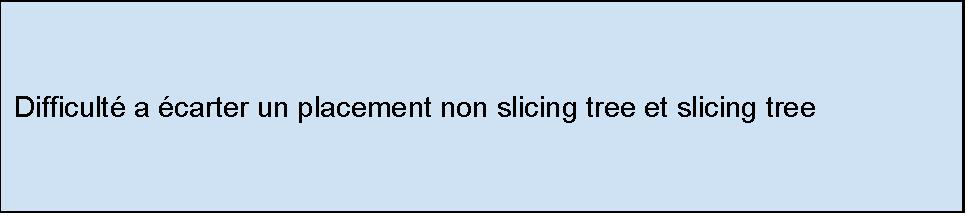
\includegraphics[height=0.10\textheight]{Figures/8.pdf}
\caption{Difficultés à écarter un placement non slicing-tree}
\label{fig:8}
\end{center}
\end{figure}
\end{itemize}
\subsection{Méthodologie de placement}
Notre méthodologie de placement consiste à effectuer un placement automatisé tout en impliquant des prises de décisions des concepteurs. L'objectif est de permettre à chaque concepteur de pouvoir appliquer ses propres contraintes sans engendrer une automatisation trop avancée. Cela entrainera des résultats moins optimisés en termes de surface mais en contre partie, le placement seront plus prévisibles et plus simplement ajustables. L'organisation de notre méthodologie se présente de la manière suivante:
\begin{itemize}
\item \textbf {La topologie en \textit{slicing tree}:} le concepteur définit une position relative des modules.
\item \textbf {Expression des contraintes de placement:} le concepteur introduit un ensemble de contraintes de placement.
\item \textbf {Algorithme de placement:} l'outil établit les placements possibles et génère un placement choisi par le concepteur.
\end{itemize}
\label{sec:Placement-methodologie}

\subsubsection{Définition d'une topologie de placement}
Lors de la conception d'un système sur puce (SoC), les espaces dédiés aux circuits numériques et analogiques sont distincts afin que chacun des circuits puissent être conçus de manière indépendante en terme de surface de circuit. Les circuits numériques sont connus pour leur structure regulière en bande dans lesquelles les cellules standards sont placées et routées sachant leurs connectivités. C'est avec cette idée de bandes que de nombreux circuits analogiques sont également organisés. Pour les circuits analogiques, ces bandes sont en revanche hétérogènes et dépendent de la hauteur des modules qui les constituent. Ces bandes ne s'étendent pas d'une extrémité à une autre du circuit mais se limitent à un groupe de modules soumis à des contraintes de proximités dû à leurs connectivités. Placer les modules de cette façon permet d'obtenir des circuits réguliers ce qui est un aspect critique pour certains circuits analogiques qui nécessitent d'évoluer dans un environnement le plus semblable possible. \newline

Avec l'objectif de représenter l'organisation en bande, nous avons opté pour le choix de la représentation des \textit{slicing trees}. Mentionné dans la section \ref{sec:Placement-SoA-topologie}, un \textit{slicing tree} est une représentation topologique qui consiste à définir un espace divisé par de nombreuses fois verticalement ou horizontalement. Ces divisions d'espace forment alors un ensemble de régions rectangulaires qui chacun peut représenter un module ou bien un espace vide pouvant être utilisé pour la phase de routage. Ces divisions sont organisées de manière hiérarchique et forment un graphe dans lequel chaque noeud hiérarchique est soit une division verticale, soit une division horizontale. Il en revient aux concepteurs la tâche de définir un \textit{slicing tree} et sa définition du \textit{slicing tree} ne sera pas altérée par notre outil de placement. Les seuls perturbations subies seront les écartements de modules afin d'y faire passer les fils de routage. En définissant eux-même la représentation topologique, les concepteurs seront libre de jugé par eux-même l'importance des contraintes de proximité, régularité ou de bordudes en fonction de l'environnement dans lequel se trouve le circuit et leurs expériences personnelles en tant que concepteur.\newline
\begin{figure}[h]
\begin{center}
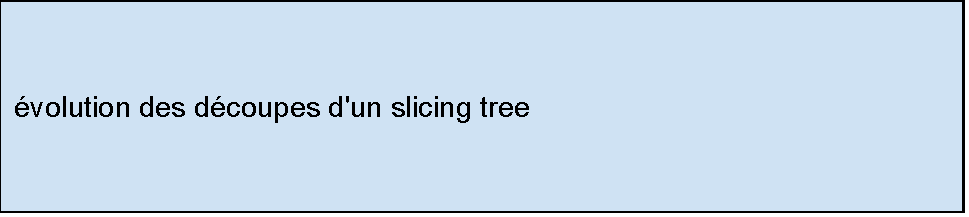
\includegraphics[height=0.10\textheight]{Figures/9.pdf}
\caption{Difficultés à écarter un placement non slicing-tree}
\label{fig:9}
\end{center}
\end{figure}\newline
\indent Fig. \ref{fig:9} présente une construction de graphe de \textit{slicing trees} pour un placement donné. On peut y observer les découpes hiéarchiques horizontales et verticales. La représentation en \textit{slicing trees} ne permet pas de représenter tous les placements possibles et un exemple de placement non représentable est donné par la figure \ref{fig:10}. Dans une certaine mesure, il est possible de représenter ces placements avec un \textit{slicing tree} mais la compaction et la surface du circuit occupées seront dégradées. Cependant, nous jugeons qu'il est plus important de prendre en compte la faisabilité du circuit en tenant compte de la capacité à espacer les modules d'un placement donné. La représentation en \textit{slicing tree} est adaptée à ces écartements, on considère que chaque découpe vertical ou horizontal puisse être un espace de routage qu'on agrandit en largeur pour une découpe verticale et en hauteur pour une découpe horizontale. \newline
\begin{figure}[h]
\begin{center}
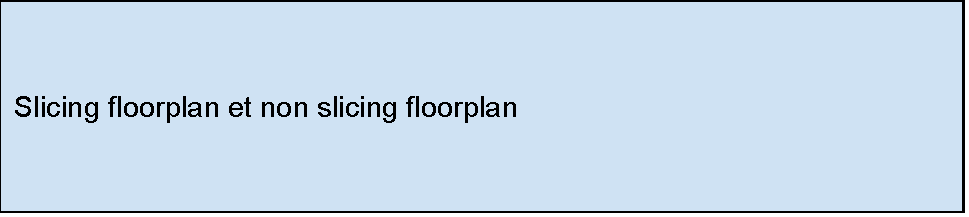
\includegraphics[height=0.10\textheight]{Figures/10.pdf}
\caption{(a) Placement représentable par un \textit{slicing tree} (b) Placement non représentable par un \textit{slicing tree}}
\label{fig:10}
\end{center}
\end{figure} 
\subsubsection{Expression des contraintes de placement}
On décompose les éléments d'un \textit{slicing trees} de la façon suivante:
\begin{itemize}
\item \textbf{les devices}
\item \textbf{les espaces de routage}
\item \textbf{Les rails traversant}
\item \textbf{les noeuds hiérarchiques}
\end{itemize}

On définit un device comme étant un bloc numérique ou analogique. Dans le cadre d'un bloc analogique, il peut s'agir d'une cellule numérique contenant une ou plusieurs cellules standards. Pour un bloc analogique, un device peut représenter un ensemble de transistors permettant de réaliser une fonction analogique de base. Ces devices peuvent être un simple \textbf{transistor}, une \textbf{paire différentielle}, un \textbf{miroir de courant}, un \textbf{montage en cascode} ou un \textbf{cross-coupled pair}. La raison pour laquelle ces blocs ont été définie est que le comportement électrique de ces blocs analogiques nécessite un dessins des masques dédié comprenant des contraintes géométriques fortes liées au placement et au routage. Ils peuvent également être générés selon des styles dessins des masques tels quepar centrage géométrique ou de manière interdigité. Ces blocs analogiques sont générés de manière correcte par construction à partir des règles de dessins de la technologie donnée. De plus, chacun des devices est paramétrable et contient les estimations des parasites liés à son dessin des masques. Pour plus de détails concernant notre librarie de devices analogiques, \cite{youssef2012} décrit entièrement le contenu de ces devices.

Dans le contexte du \textbf{slicing tree}, un device est défini par plusieurs attributs:
\begin{itemize}
\item \textbf{Une coordonnée x, y}: Elle représente la position du coin inférieur gauche du device au sien du plan considéré pour le placement des devices.
\item \textbf{Une hauteur et une largeur}: Elle définit le rectangle englobant la surface occupée par le device.
\item \textbf{Une contrainte d'alignement}: Elle positionne le device au sein du noeud hiéarchique, d'avantage de détails seront donnés dans la description d'un noeud hiéarchique. 
\item \textbf{Variation du nombre de doigts des transistors}: Les configurations en nombre de doigts de transistors tolérées par le concepteur.
\end{itemize}

\begin{figure}[h]
\begin{center}
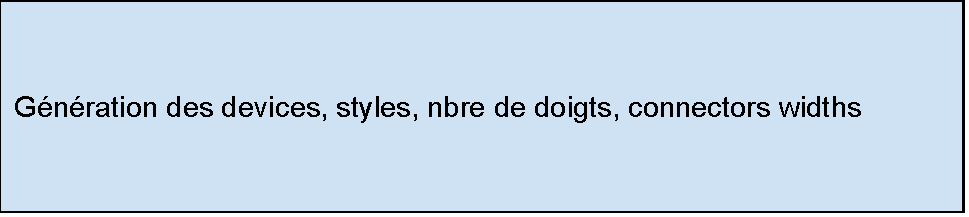
\includegraphics[height=0.11\textheight]{Figures/12.pdf}
\caption{Les paramètres réglables des devices, (a) Style de dessin des masques, (b) Variation du nombre de doigts et (c) Variation de la taille des connecteurs.}
\label{fig:12}
\end{center}
\end{figure} 
Notre approche de placement consiste à organiser les devices en bande et on cherche également à faire sorte que les devices d'une bande possèdent une hauteur le plus similaire possible. Afin d'obtenir cette configuration, il est nécessaire de considérer plusieurs aspect ratios pour chacun des devices en faisant varier le nombre des doigts des transistors des blocs analogiques tout en préservant leur fonctionalité électrique. Néanmoins, nous sommes conscient que cette action implique une variation de la capacité source/drain $C_{jSB}$ pouvant influencer les performances du circuits. \cite{Long2006} et \cite{Wu2014} détaille cette influence de la variation du nombre de doigts d'un transitor. Cependant, dans le cadre de notre approche, notre objectif consiste à effectuer plusieurs boucles itératives sur l'ensemble du design et ainsi resserrer les contraintes du circuit à chaque nouvelle itération afin de tendre vers une solution souhaitée. \newline
 
\indent Les espaces de routage sont des espaces vides dédiés au positionnement des fils de routage. Au sein d'un \textbf{slicing tree}, chaque découpe du circuit est considéré comme un espace de routage rectangulaire redimensionnable dans une seule direction. Dans le cas d'une découpé verticale, l'espace de routage peut être redimensionné de manière horizontale et on appelle ces espaces comme étant des espaces de routage verticaux. Réciproquement pour les découpes horizontales, l'espace de routage peut être redimensionné manière verticale et on appelle ces espaces comme étant des espace de routage horizontaux. Les espace de routage représentant une découpe du \textbf{slicing tree} sont implicites et ne nécessitent pas d'être précisé par l'utilisateur. Pour des raisons de clareté, les espaces de routage dûs à une découpe du \textbf{slicing tree} ne seront pas représentés sur un \textbf{slicing tree}. En revanche, il est possible de considérer des espaces vides volontaires rectangulaires, ces derniers peuvent être utilisés pour des ajustements de position.\newline

\indent Dans le contexte du \textbf{slicing tree}, un espace de routage est défini par plusieurs attributs:
\begin{itemize}
\item \textbf{Une coordonnée x, y}: Elle représente la position doi inférieur gauche de l'espace de routage au sien du plan considéré.
\item \textbf{Une hauteur ou une largeur}: Elle définit l'épaisseur de la découpe (largeur pour une découpe verticale et hauteur pour une découpe horizontale).
\end{itemize}
\begin{figure}[h]
\begin{center}
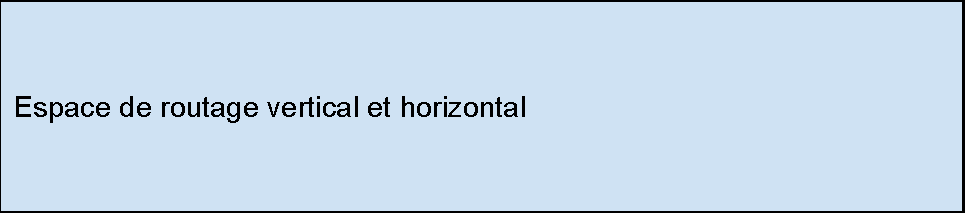
\includegraphics[height=0.11\textheight]{Figures/13.pdf}
\caption{Espace de routage vertical et horizontal}
\label{fig:12}
\end{center}
\end{figure} 

Les noeuds hierarchiques représentent les découpes hierarchiques verticales et horizontales du circuit. Ces noeuds permet la gestion des contraintes appliqués aux devices tels que les contraintes d'alignement et gèrent également les contraintes de symétries des devices. Chaque noeud hiéarchique possède des noeuds fils pouvant être des devices, des espaces de routage, des rails ou un autre noeud hierarchique et gère la propagation des contraintes soumis par le concepteur vers les racines du \textbf{slicing tree} ainsi qu'aux espaces de routage implicites dûs aux découpes. Les noeuds hierachiques propagent également les aspects ratios des devices en \textbf{bottom-up} jusqu'à la racine du \textbf{slicing tree} qui représente les aspects ratios globales du circuit. \newline

\indent Dans le contexte du \textbf{slicing tree}, un noeud hiéarchique est défini par plusieurs attributs:

\begin{itemize}
\item \textbf{Une coordonnée x, y}: Elle représente la position du coin inférieur gauche de l'espace occupé par le noeud hiéarchique et ses noeuds fils.
\item \textbf{Une hauteur et une largeur}: Elle définit le rectangle englobant la surface occupée par l'espace occupé par le noeud hiéarchique et ses noeuds fils.
\item \textbf{Une contrainte d'alignement}: Elle positionne le noeud hiérarchique au sein du noeud hiéarchique supérieur.
\item \textbf{Ensemble de noeuds fils}: L'ensemble des noeuds fils est stocké dans un ordre déterminé déterminant le positionnement.
\item \textbf{Les symmétries}: Les noeuds fils symétriques sont stockés au niveau du noeud parent.
\item \textbf{Paramètre de validité}: La différence de taille entre device est souvent importante. Afin de se rapprocher le plus possible d'une topologie en bande, ce paramètre permet de spécifier la différence de taille autorisé pour considérer la bande comme étant un placement valide.
\end{itemize}
\begin{figure}[h]
\begin{center}
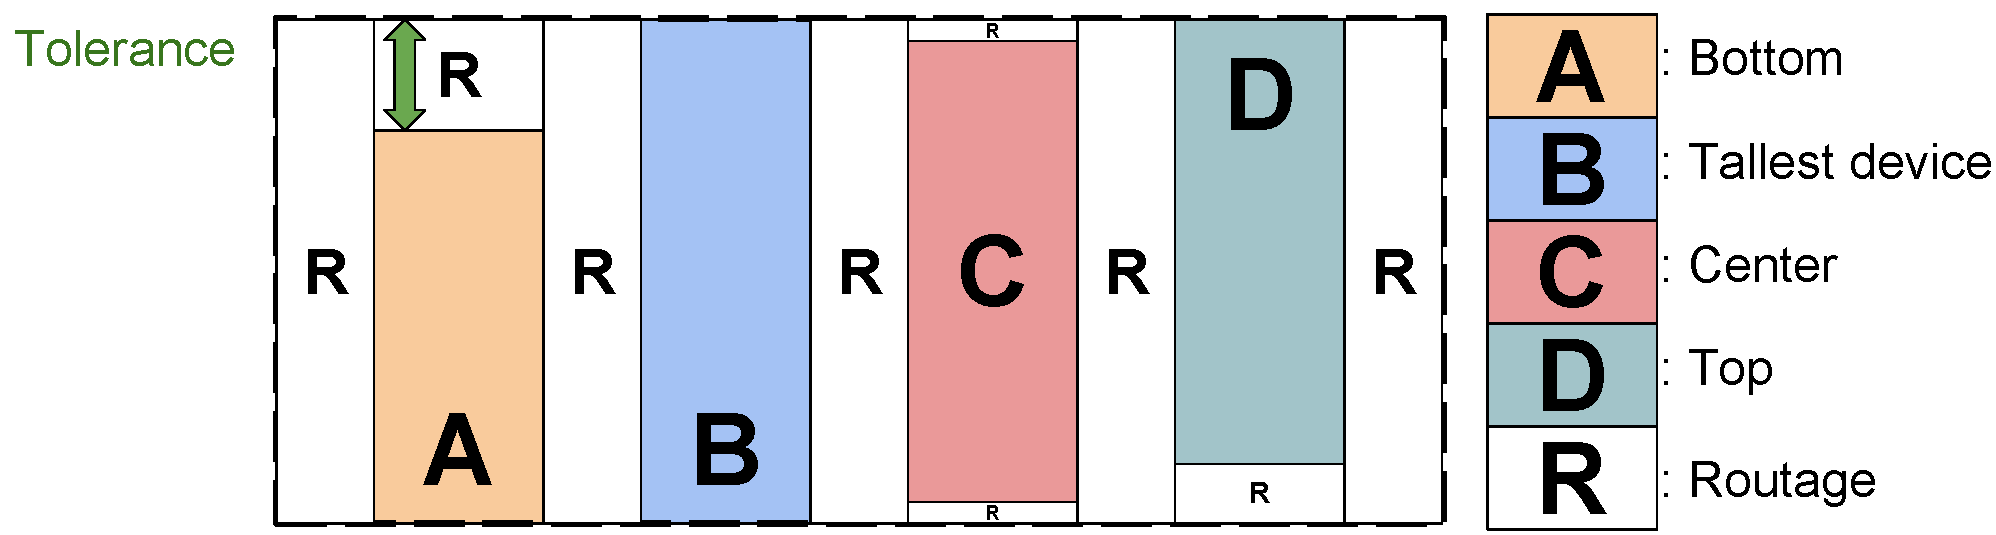
\includegraphics[height=0.15\textheight]{Figures/14.pdf}
\caption{Noeud hiérarchique vertical avec une organisation en bande}
\label{fig:14}
\end{center}
\end{figure} 

La figure \ref{fig:14} présente l'organisation d'un noeud hiérachique vertical. On y observe l'organisation d'une bande dans laquelle les devices $A$, $B$, $C$ et $D$ sont soumis à des contraintes d'alignement. La hauteur et la largeur d'un noeud hiérarchique vertical est déterminé par la formule suivante:
\begin{equation}
\begin{aligned}
Largeur_{BandeVerticale} &= \sum_{i=0}^{n} L_{NoeudFils_i} + \sum_{j=0}^{n+1} L_{EspaceDeRoutage_j} \\
Hauteur_{BandeVerticale} &= Max\{H_{NoeudFils_0},H_{NoeudFils_1}, ... , H_{NoeudFils_n}\}
\end{aligned}
\end{equation}
en considérant $n$ le nombre total de noeuds fils. Chaque espace noté "$R$" représente un espace de routage et sont dû soit à une découpe verticale soit à une différence de taille avec le noeud fils ayant la plus grande hauteur qui est "$B$" dans le cas ci-dessus. La taille d'un espace de routage dépend du nombre de fils de routage verticaux et de leur positinnement au sein de l'espace, d'avantage de détails seront donnés dans le chapitre sur le routage. Concernant les contraintes d'alignement à chacun des devices, "$A$" est aligné vers le bas de la bande, "$C$" est centré par rapport à la hauteur de la bande et "$D$" est aligné vers le haut de la bande. Les symétries au sein d'un noeud hierarchique se traduisent par la garantie que deux fils d'un noeud fils soient de la même taille et possède le même alignement. Sur la figure \ref{fig:14}, la boite englobante en pointillé représente l'espace du noeud hiéarchique considéré par les noeuds hiearchiques supérieurs.


\begin{figure}[h]
\begin{center}
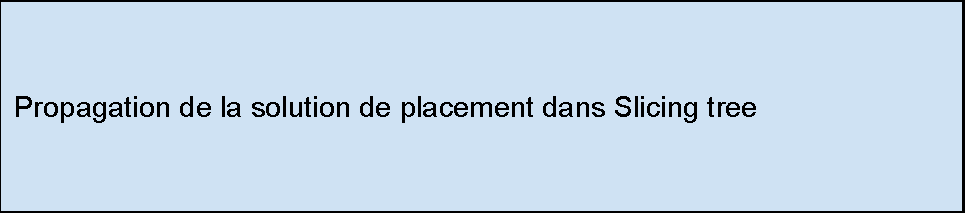
\includegraphics[height=0.11\textheight]{Figures/15.pdf}
\caption{Propagation des dimensions du placement dans un \textbf{slicing tree}}
\label{fig:11}
\end{center}
\end{figure} 

\begin{figure}[h]
\begin{center}
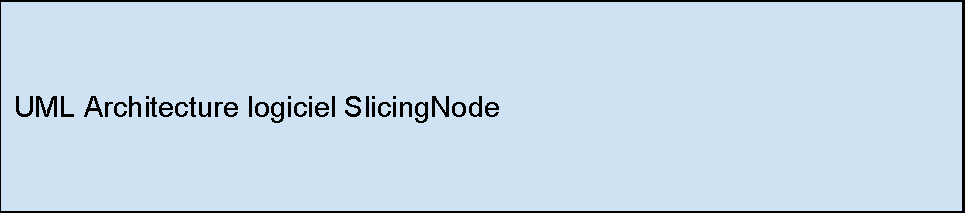
\includegraphics[height=0.11\textheight]{Figures/11.pdf}
\caption{Interface de programmation du placeur analogique et mixte}
\label{fig:11}
\end{center}
\end{figure} 

Je fais un test
- API SlicingTree: Architecture logiciel ~1 page
- SlicingNode: 
DSlicingNode: NodeSets (number of fingers, dimensions), definition of what we call device? Layout style?
RoutingNode : Width of the channel, variable length depending on vertical or horizontal nodes
HSlicingNode et VSlicingNode: containing DSlicingNode, modificateur/accesseur (add, remove, find)
get Width/Height
slicing routing
adjust border slicing routing

Symmétries:
- symmetries inside a same level of hierarchie
- 2 blocks can be set to have the same dimensions

\subsubsection{Algorithme de placement}

How
- variation devices, layout styles
- Margin tolerances: Imposer des contraintes afin de limiter le nombre de placement possible
- Algorithme de calcul du nombre de placement possibles + Execution HVState ?
- Placement + stored placement

\section{Exemples}
\label{sec:Placement-Exemple}
What
- gmchamla
- Expliquer la structure de la description python
- Etapes à suivre avec l'execution des outils + screen des étapes
- Interface graphique, choix des positions et parametres de selections
- Différents résultats de placement à montrer
\section{Conclusion}
\chapter{Problem Definition}
An automatic placement tool should produce analog device-level layouts similar in density and performance to the high-quality manual layouts. Having the devices for the selected topology sized, they must be laid out in the chip. Considering these devices and their interconnects, the problem is to explore non-overlap placements of given modules. The capability to deal with layout constraints, in order to eliminate unwanted parasitics due to the process variations, is mandatory. cite{00} enumerates the most common placement constraints that are respected by modern analog placer. Among them, symmetries and symmetry-island cite{3} are the most used constraints. Other constraints like common-centroid cite{4}, proximity and range are also often considered cite{5}. Taking into account current and signal path improves performance accuracy cite{6}. Devices can be placed depending on their thermal impact on the chip cite{7}. Regularity cite{8} and boundary constraints cite{9} enhance routability and suppress parasitics induced by extra bends of wires and via cost.
\newline 
\newline 
\indent Given a placement of a set of layout devices together with their positions, the layout must then be interconnected according to the netlist in a design rule correct way. Due to the fact that the performances of an analog circuit are critically dependent on layout parasitics, the routing of an analog circuit requires more attention than that of a digital circuit. Analog routing constraints can be critical such as symmetry, topology and wirelength matching.
\newline 
\newline 
\indent Recent research focused on using simulated annealing algorithm (SA) in combination with topological representations to respect these placement constraints. Topological representations encode the positioning relations between devices and SA optimizer alters their relative positions. The most popular representations used in analog placement over the last decades are Sequence-Pair cite{10}, B*-Tree cite{11}, Transitive Closure Graph cite{12}, Ordered-Tree cite{13} and slicing floorplans cite{15} and they were coupled with some constraints to respect at the same time. This will be discussed in the following section
% \newline 
% \newline 
% \indent Although most of the recent works focus on simulated annealing algorithm cite{00}, we believe that giving more control to the designer and using his interventions to set some constraints yields good analog placement results. Our approach introduces a semi-automatic analog placement approach guided by the designer's preferences. This semi-automatic approach also helps the designer to debug more efficiently and make adjustments easier since he will, himself, control the overall relative placement of the circuit but at the same time, some tiresome and error-prone tasks are automated. 
\chapter{State of the Art}
Analog layout automation tools follow different approaches. Procedural generation tools are about codifying the entire circuit layout using parametric representation by the designer through a procedural language or graphical user interface. Template-based tools incorporate designer knowledge into the optimization task. This approach finds its applications restricted to small circuits or to more complex circuits with the goal of achieving the first cut design. Optimization-based tools use iterative procedure where design variables are updated at each iteration until they achieve an equilibrium point. Overall successful layout generation tools are often optimization-based.
\newline 
\newline 
\indent cite{20} reviews characteristics that can be taken into consideration to evalutate automation tools:
\begin{itemize}
\item \textit{Accuracy and robustness}: Measure of the tool's performance prediction compared to real performance 
and capacity of the tool to build and test circuits tolerant to
manufacturing faults and operating point variations.
\item \textit{Automation level}: Time spent to design a circuit with the tool. We can consider the running
time (time spent by the tool to provide a solution) and the setup time
(time spent by the designer to adequate the problem to the tool).
\item \textit{Scope of the tool}: It can be described as a group of analog design problems, which can be
solved by this tool. A tool which aims at solving a wide range of design
problems will be successful in the long run.
\item \textit{Design facilities}: Multi-objective optimization, interactive design, bookkeeping facilities.
\end{itemize}
\chapter{Academic Tools}
Some academic tools related to analog layout generation will be reviewed in this following part. 
\newline 
\newline 
\indent Examples of procedural generation tools:
\begin{itemize}
\item ALSYN cite{21} can synthesize layout from netlist-level description for a range of analog integrated circuits. Designers can incorporate their own reusable knowledge into the synthesis process to explore design space. It also provide a flexible module generator environment and easy technology database access with variable shapes.
\item cite{22} describes the automatic generation and reusability of physical layouts of analog and mixed-signal blocks based on high-functionality parameterized cells (pCells) that are fully independent of technologies.
\end{itemize}

Examples of template-based tools:
\begin{itemize}
\item LAYGEN cite{24} is template based tool that includes placement and routing constraints defined by the designer following a traditionnal analog flow that can generate automaticaly analog integrated circuit layouts.
\item BAG cite{23} is a design frame for AMS circuits capable of integrating all steps of the design flow, from architectural-specification definition to correct layout implementation, into procedural analog generators.
\end{itemize}
Examples of optimization-based tools:
\begin{itemize}
\item ANAGRAM cite{25} is a full-custom layout of analog cells which is in the style of a macro-cell place and route problem. It can handle layout symmetries, dynamic merging and abutment of individual devices, and flexible generation of wells and bulk contacts
\item ILAC cite{26} is process-independent tool that automatically generates geometrical layout for analog CMOS cells from a circuit description. It handles typical analog layout constraints such as device matching, symmetry and distance and coupling constraints but also supports user-specified constraints.
\end{itemize} 
\chapter{Industrial Tools}
Some industrials tools related to analog layout generation will be reviewed in this following part.
\begin{itemize}
\item Synopsys Helix (ex-Ciranova since 2012) cite{27} is a device-level automated placement solution for analog, and mixed-signal IC designs such as PLLs, SerDes, ADCs and PHYs. Helix is fully hierarchical and offers capacity in the tens of thousands of transistors, enabling it to optimize floorplanning and placement for
entire custom IC blocks or IP at once.
\item Mentor Graphics Pyxis Layout Suite cite{28} offers configured options for design engineers who need increased productivity and an automated way of handling the physical layout of their AMS designs. Bundles are offered in a standard configuration, with optional applications that provide increasing levels of automation and functionality to address the designers unique requirements.
\item Synopsys Laker cite{29} delivers a complete solution for analog, mixed-signal, and custom digital design and layout that is optimized for performance and interoperability for 28-nanometer (nm) and below design flows. It has a built-in understanding of analog layout requirements, so it is much easier to adopt and deploy than competing analog automation tools.
\item Virtuoso Layout Suite Family cite{30} comprises the layout environment of the industry-standard Virtuoso custom design platform, a complete solution for front-to back custom analog, digital, RF, and mixed-signal design. It preserves design intent throughout the entire physical implementation process, while managing multiple levels of design abstractions from device, cell, and block levels through to the full-chip level.
\item Tanner EDA - High Performance Device Generation (HiPer DevGen) cite{31} creates building blocks based on an understanding of the functional requirements that are needed to produce a high-quality layout. Retargeting the components to a new technology node simply requires the user to input the manufacturing rules for that technology and regenerate the devices and primitives.
\end{itemize} 
\chapter{Challenges}

Although most of the recent works focus on simulated annealing algorithm cite{00}, we believe that giving more control to the designer and using his interventions to set some constraints yields good analog placement results. Our approach introduces a semi-automatic analog placement approach guided by the designer's preferences. This semi-automatic approach also helps the designer to debug more efficiently and make adjustments easier since he will, himself, control the overall relative placement of the circuit but at the same time, some tiresome and error-prone tasks are automated.
\newline 
\newline 
\indent Another critical part in analog design, that has not been considered in most of the previous work, is the routing phase. Conventionally, the execution of placement and routing has been sequential. If the routing is a two-step procedure, the execution of the global routing and detailed routing is also sequential. Simultaneous performance optimization of the placement and the global routing can lead to a more accurate search and this is what we aim to do unlike most of the recent research who only consider the placement alone. The general reluctance of analog designers toward using automatic layout generation tools is because they are skeptical about their reliability and they would like to have full control over the layout generation process. They would prefer the layout tool to be an assistant to them and generating a template for the layout is sometimes better for them.
 
\chapter{Analog/Mixed-signal Design Approach}
\begin{figure}[h]
\begin{center}
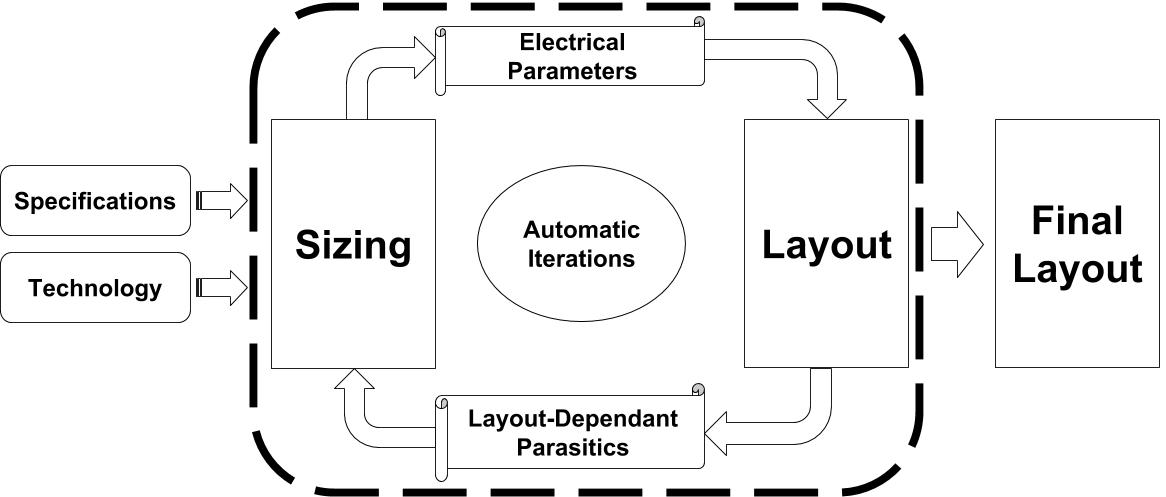
\includegraphics[height=40mm]{Figures/3.jpg}
\caption{Cairo Hurricane AMS Design Flow}
\end{center}
\end{figure}
\vspace{-1.5cm}
\section{Design Flow}
The Cairo Hurricane AMS (CHAMS) project cite{002}, developed by the LIP6 Laboratory, proposes a complete flow which would be able to create a library of reconfigurable analog Intellectual Properties, to automatically generate and optimize the layout with little intervention from the designer. The flow provides a reliable and efficient solution taking into account parasitic effect-aware layout generation with enough flexibility to adapt to different designers needs and concerns. CHAMS layout generation tool supports any technology with the new nanometric layout dependent parasitic parameters.
\newline 
\newline 
\indent The proposed CHAMS analog design (Fig. 2) is a two way communication between the sizing and layout generation. The idea is that the sizing tool provides the electrical parameters of the transistor such as the width, length, number of fingers, etc... to the layout generation tool. The tool automatically generates the layout from a library of parameterized cells and sends back to the sizing engine the layout-dependent parasitic parameters such as the drain and source areas and perimeters, the stress effect parameters, etc... to re-evaluate the performance. This internal loop is repeated several times, with minimal designer intervention, until the target specifications are met.
\newline 
\newline 
\indent Our goal is to develop a tool capable to place and route analog layout respecting designer specifications in a shorter amount of time compared to the fully manual approach. We also aim to have a tool which will be technology independant and can as well, place  and route mixed-signal circuits. At this moment, the bottleneck of our design flow is to handle analog place and route and this is the reason why this thesis is mainly focused on it.
 
\section{Placement in row}
Digital and analog circuits have a dedicated area on a system-on-chip circuit so they can be independently designed within a specific space. Digital circuits are well-known for their regular row structure where standard cells are placed and routed accordingly to their netlist. In a similar way, we plan to organize the analog circuit layout in rows of devices and the analog circuit area should be placed and routed within its dedicated area. 
\newline 
\newline 
\indent It is common to design analog circuit in rows of devices where the height of each row of devices should be adjustable so it can match its dedicated area. Therefore, we choose the slicing tree representation for several reasons:

\begin{itemize}
\item Slicing trees are a natural choice since they are adequate to the row structure. Rows are represented by horizontal slices which will be divided into vertical slices determined by the area of each device.

\item Unlike most of modern analog placement methods, our placement strategy is semi-automatic and will be guided by the designer's preferences. Slicing trees are easy to handle and let the designer choose the overall topology. That shows some advantages that will be explained in the following section.
\end{itemize}    
\chapter{Methodology for the placement}

Modern analog automation tools are able to generate analog layout respecting various placement constraints and they mainly use simulated annealing approach. Nevertheless, such approach might not produce predictable and easy-to-adjust results. We believe that giving more control to the designer will generate analog layout, easier to predict compared to optimization-based approach, but also easier to adjust in case modifications are required. Our analog/mixed-signal placer is semi-automatic: the device generation is automated and generated correct-by-construction and guided by the designer's constraints over the circuit. The following sections will describe the interventions from the designer.

\begin{figure}[h]
\begin{center}
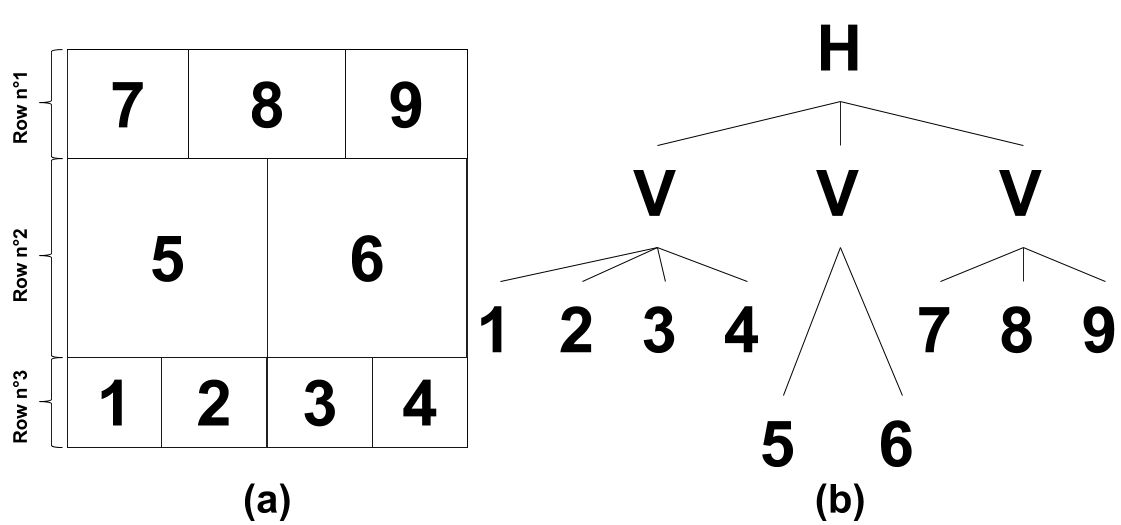
\includegraphics[height=50mm]{Figures/1.png}
caption{Example of placement (a) and its slicing tree representation (b) where "H" stands for horizontal cut and "V" for vertical cut}
\end{center}
\end{figure}
\vspace{-1cm}
\section{Slicing Tree Construction}
In order to organize devices in row, we use the slicing tree structure (Fig. 3) which will be described by the designer and not automatically generated by the placer. Our placer will only assist the designer so it generates the slicing tree according to the designer's constraints. A slicing tree is a slicing floorplan that represents an area that has been divided multiple times either vertically or horizontally, forming a set of rectangular regions representing the place filled by each device. These slices are organized hierarchically so they form a graph where the hierarchical node are either horizontal or vertical cuts. Fig. 3 shows an example of a slicing tree representing a circuit of 9 devices organized in three rows.

\section{Devices Variations}
Our placement approach consists in organizing devices in row, that is to say to have rows of devices with similar height, and the overall analog part's height would be a multiple of standard cell's heights from the digital circuit part. To obtain a row of devices, the height of each device needs to be similar and this is the reason why, we need to consider several possible aspect ratios for each device by varying the number of fingers (Fig. 4) like in cite{6} so we can find heights of devices that match a given height. 
\newline 
\newline 
\indent However varying the number of fingers of a MOS transistor implies a variation of the source/drain capacitance $C_{jSB}$ which can impact the circuit performance. This variation can be calculated using the formula \eqref{1}:

\begin{figure}
  \begin{minipage}[c]{.48\linewidth}
    \begin{center}
      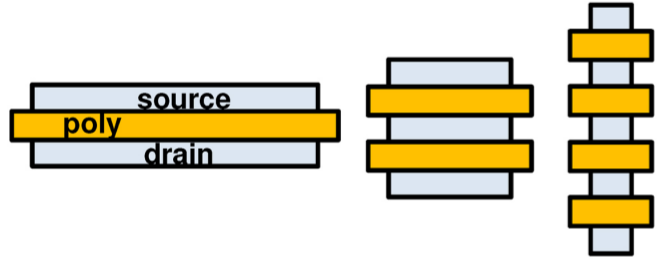
\includegraphics[width=80mm]{Figures/5.png}
      caption{MOS transistor with different finger numbers resulting in different physical dimensions}
    \end{center}
  \end{minipage} \hfill
  \begin{minipage}[c]{.48\linewidth}
    \begin{center}
      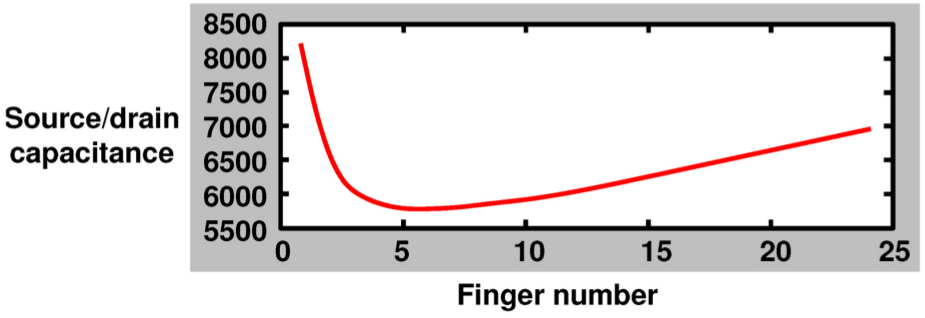
\includegraphics[width=80mm]{Figures/4.png}
      caption{Induced source/drain capacitance of a MOS transistor function cite{6}}
    \end{center}
  \end{minipage}
\end{figure}

\begin{equation}\label{1}
C_{jSB} = \frac{A.C_j}{\Big(1-\frac{V_{BS}}{\phi _j}\Big)^{m_j}}+\frac{P.C_{jsw}}{\Big(1-\frac{V_{BS}}{\phi _j}\Big)^{m_{jsw}}}
\end{equation}
with:
\begin{itemize}
  \setlength\itemsep{0em}
\item $A$ and $P$: source/drain Area and Perimeter
\item $C_j$ and $C_{jsw}$: Bottom and Sidewall junction capacitances 
\item $\phi _j$: built-in junction potential
\item $m_j$ and $m_{jsw}$: depend on the doping profile of the junction
\end{itemize}

Considering a given MOS transistor, its channel width and length is decided by the sizing step and cite{6} presents the following formula of $C_{jSB}$ variation based on the number of fingers:

\vspace{-0.5cm}
\begin{equation}
C_{jSB}(F) = (\alpha .W.L+\alpha .W.\delta _{gap} + 2.\beta .\delta _{gap})+2.\beta .F(L+W.\delta _{gap})+\frac{W}{F} (\alpha .\delta _{gap}+2.\beta)
\end{equation}
with:
\begin{itemize}\label{2}
  \setlength\itemsep{0em}
\item $F$: number of fingers
\item $W$ and $L$: channel Width and Length
\item $\alpha = \Big(1-\frac{V_{BS}}{\phi _j}\Big)^{m_j}$
\item $\beta = \Big(1-\frac{V_{BS}}{\phi _j}\Big)^{m_{jsw}}$
\item $\delta _{gap}$: gap seperating 2 fingers 
\end{itemize}

As cite{2} mentioned, changing the number of fingers of a device can considerably change the source/drain bulk capacitance (Fig. 5) and therefore the device properties. Nevertheless, as mentioned in section 4.1, our placement phase is part of an internal loop, which is repeated until a result meets the required performances (Fig. 2). Also, it is the task of the designer to decide the admissible range of shapes for every device which would limit the number of finger variations.

\section{Margin Tolerances}
We aim at creating rows and it is important to define what we consider as a row of devices. We introduce a tolerance margin, which represents the difference between the smallest and the tallest device's height in a vertical node. Fig. 6 (a) shows an example of devices organized in row where the area A, B, C and D represent devices. Devices A and B show respectively the smallest and highest height inside the row. This difference of height is compared to the tolerance parameter to establish if this is considered as a legal row. We apply the same concept to the horizontal node but instead of using the height as a comparison, we use the width. It is up to the designer to adjust this tolerance margin and it will impact on the number of accepted possibilities. Different margin tolerances can be considered at each hierarchical nodes. At the same time, having a small tolerance will reduce the waste of space induced by the slicing tree representation.

\begin{figure}[h]
\begin{center}
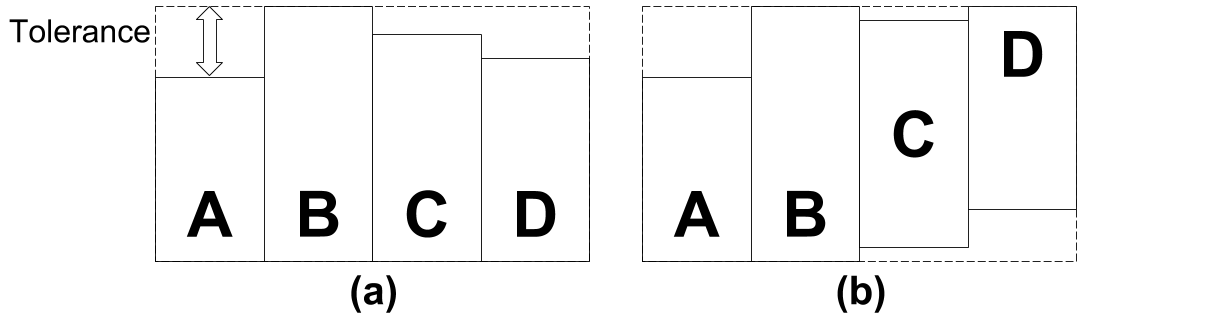
\includegraphics[height=30mm]{Figures/2.png}
caption{Tolerance (a) and alignment (b) in slicing tree representation}
\end{center}
\end{figure}
\vspace{-1cm}
\section{Placement Constraints}
As said in section 3.1, it is the task of the designer to describe the slicing tree with the help of our placer. This will directly impact on the topology of the circuit. This means he will have the total control over the relative relation between the blocks. Having the designer building his own slicing tree also means that he will have control over placement constraints such as proximity, boundary, current/signal path and regularity constraints based on his knowledge and preference.
\newline 
\newline 
\indent Among the most common constraints, symmetries can be respected with the appropriate slicing tree organization. We also consider alignment constraints inside of a slicing tree in horizontal or vertical node. In Fig. 6 (b), we have an example of possible alignments: devices A and B are aligned to the bottom of the row, device C is centered and device D is aligned to the top of the row. In horizontal slices, devices can be aligned to the right, center and left of the row.

\section{Placement Choice}
Similar to cite{17}, once all the possible variations are set for each device, we evaluate the accepted variations at hierarchical nodes based on the margin tolerances. These accepted variations are propagated from the bottom of the slicing tree to the root. After this bottom-up propagation, the designer processes the different placements based on height, width or global ratio criteria. He can choose the most optimized placements according to the Pareto front curve like in cite{18}, but he is free to choose any other possible placement that would eventually have more white space if the circuit can afford more space. 
\chapter{Placement Algorithm}
\section{Theory}
{\bf \noindent  Definition 1:} \\
Considering $n$ nodes for a Vertical hierarchical node (Fig. 6) with $n$ representing the number of children, its height and the width are calculated with the following formulas: \\
\vspace{-0.5cm}
\begin{subequations}
\begin{align}
Height &= max(Height_{Node_1}, Height_{Node_2}, \hdots, Height_{Node_n})\\
Width  &= \sum_{k=1}^{n} Width_{Node_k} 
\end{align}
\end{subequations}
For a Horizontal hiearchical node, we have:
\vspace{-0.25cm}
\begin{subequations}
\begin{align}
Height &= \sum_{k=1}^{n} Height_{Node_k} \\
Width  &=  max(Width_{Node_1}, Width_{Node_2}, \hdots, Width_{Node_n})
\end{align}
\end{subequations}
{\bf \noindent  Definition 2:} \\
Each $Node_X$ has $m$ pairs (height, width) representing the size that it can take, unless if the node is preset. When a node is preset, it has a single size height/width defined by the designer:

\begin{algorithm}
\caption{Possible sizes}
\eIf{$Node_X$ is preset}{
  $Node_X: [(Height_{\textit{preset}}, W_{\textit{preset}})]$
}{
  $Node_X: [(Height_1, Width_1), (Height_2, Width_2),\hdots ,(Height_m, Width_m)]$\\
  with $m$, number of sizes\\  
}
\end{algorithm}
The algorithm evaluates all the possible sets if they can be accepted based on the tolerance margins parameter for the height and the width of the hierarchical node. It starts with the first possible sizes of each node:

\begin{algorithm}
Initial set:\\
\begin{equation}
  HierarchicalNode (Height_1, Width_1) = 
  \begin{pmatrix}
    Node_1(Height_1, Width_1)  \\
    Node_2(Height_1, Width_1)  \\
    \vdots            \\
    Node_n(Height_1, Width_1)  
  \end{pmatrix}
\end{equation}\\
\end{algorithm}
\vspace{-0.5cm}

Once this set of pairs height/width is processed, $Node_1$ considers then its second size $(Height_2, Width_2)$ until all its possible sizes are considered. Once the last size is reached for $Node_1$, $Node_2$ passes to its second size and $Node_1$ back to its first possible size and so on. The main algorithm is the following one:

\begin{algorithm}
\caption{Main Placement Algorithm}
{\bf Case:} Vertical Node \\
\For{i = 1:Number of sets}{\vspace{0.25cm}
  Determine $(Height_{max_i}, Height_{min_i}, Width_{i})^{(1)}$\vspace{0.25cm}\\
  \If{ $(Height_{max_i} - Height_{min_i}) <=$ \textit{Height tolerance}$^{(2)}$ } 
  {Accept size $(Height_{i}, Width_{i})$} 
 
}\vspace{0.25cm}

{\bf Case:} Horizontal Node \\
Same algorithm except for $(1)$ and $(2)$.\\
$(1)$: Determine $(Width_{max_i}, Width_{min_i}, Height_{i})$\\
$(2)$: $(Width_{max_i} - Width_{min_i}) <=$ \textit{Width tolerance}\vspace{0.25cm}
\end{algorithm}
\newpage
The total number of sets to be evaluated is: 
\vspace{-0.25cm}
\begin{equation}
\textit{Number of sets} =  (m_{Node_1} * m_{Node_2} * \hdots * m_{Node_n})\\
\end{equation}

The number of sets to consider may seem to grow at a fast rate but some considerations need to be taken into account. Inside of a slicing tree, it is very common to have several hierarchical nodes which implies that some sets will be filtered by the condition $(2)$ of the main placement algorithm (Algorithm 2) for not respecting the margin tolerances. Moreover, a hierarchical node can contain symmetries between its children nodes. It means that for 2 symmetrical nodes, only $m$ possible sizes will be considered instead of $m^2$. 

\section{Results}

\begin{figure}[h]
\begin{center}
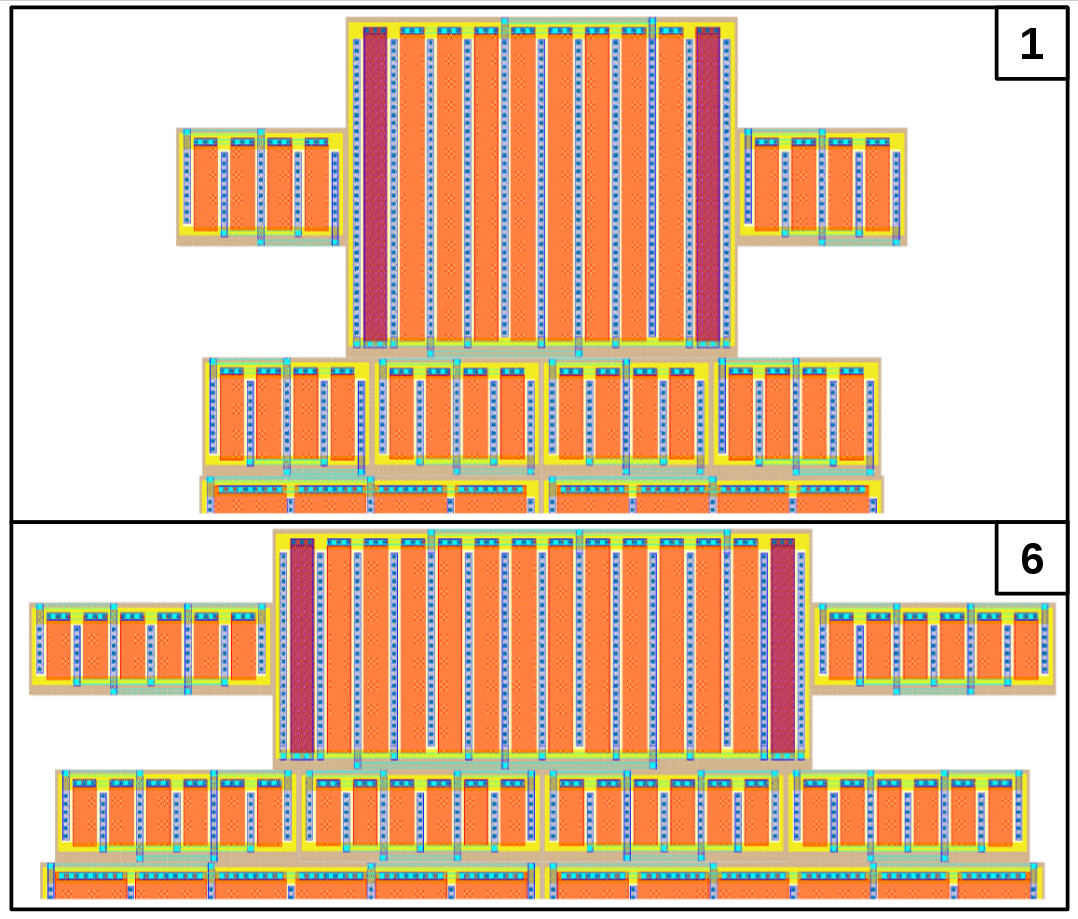
\includegraphics[width=80mm]{Figures/zoom.jpg}
\caption{Evolution of 2 rows from layout 1 and 6 of Table II for different global aspect ratios. These figures have the same scale.}
\end{center}
\end{figure}
\vspace{-0.5cm}

\begin{figure*}[t]
\begin{center}
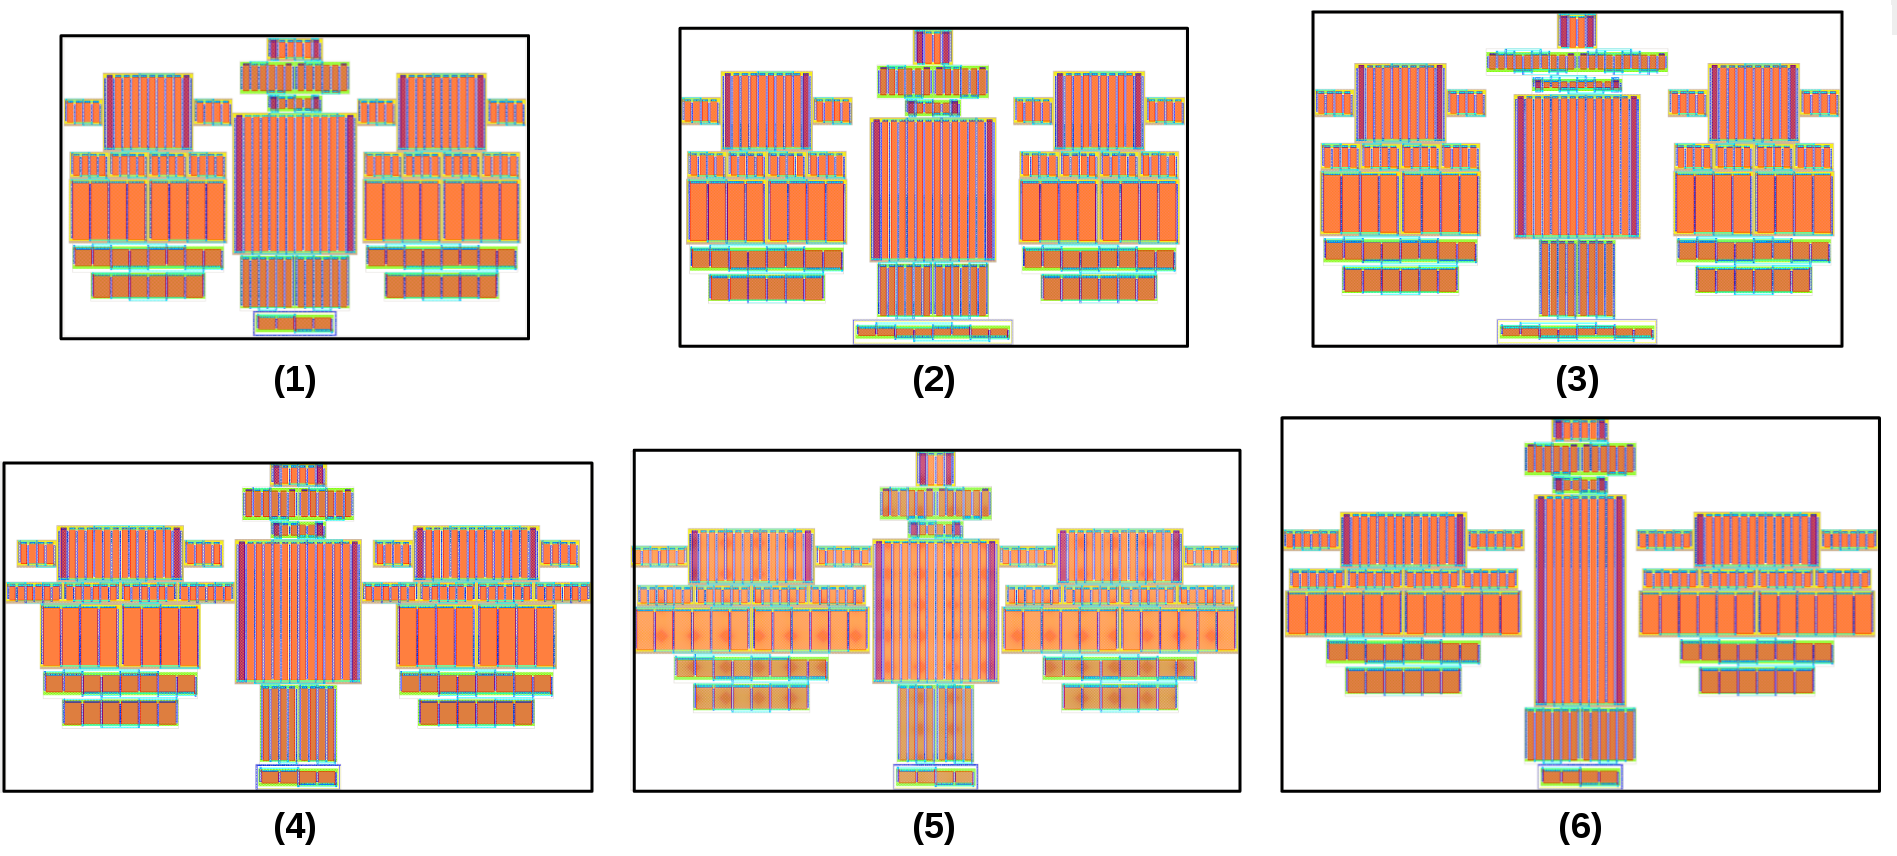
\includegraphics[width=150mm]{Figures/all.png}
\caption{Layouts of the fully differential transconductor cite{19} from Table II. These figures have all the same scale.}
\end{center}
\end{figure*}
Our placement algorithm was implemented in C++ programming language on a Intel(R) Core(TM) i5-4590S CPU @ 3.00 GHz workstation with 6 GB RAM. To illustrate the capability of our algorithm, we experiment it on a fully differential transconductor cite{19}, designed under a technology CMOS 130 nm.
\newline 
\newline 
\indent  The fully differential transconductor is composed of a total of 32 devices and we consider 2 possible variations for each device. The slicing tree takes into account 11 symmetries for this circuit and tolerance margins are set in a way to have reasonnable amount of accepted possibilities. Our algorithm found 384 possible placements in less than 1 second, some of them are listed on Table II and can be seen on Fig.8.
\newline 
\newline 
\indent  Table II shows the characteristics of those layouts with their total area, their width, their height and the percentage of the circuit occupation in the total area. Fig. 7  and Fig. 8 illustrate the layouts described in Table II and show the evolution of the rows for different global aspect ratios. The designer can choose his final placement based on his experience and preference. The placement results are plotted on a graph with heights and widths as axis and can be selected interactively to be placed in a few seconds.

\begin{table}[h]  
\caption{Some layout results of the fully differential transconductor}
\begin{minipage}{9cm}
\begin{tabular}{|C{2.5cm}|C{3cm}|C{3cm}|C{3cm}|C{2.5cm}|}
\hline
Layout & Area ($\mu m^2$) & Width ($\mu m$) & Height ($\mu m$) & Occupation ($\%$)\\
\hline
1 & 4600 & 84 & 54 & 68 \\
\hline
2 & 5116 & 91 & 57 & 63 \\
\hline
3 & 5603 & 94.2 & 59 & 58 \\
\hline
4 & 6162 & 105 & 59 & 52 \\
\hline
5 & 6648 & 109 & 61 & 49 \\
\hline
6 & 7105 & 107 & 67 & 46 \\
\hline
\end{tabular}
\end{minipage}
\end{table} 
\chapter{Future Work: Routing}

Once the placement phase is performed with the slicing tree, it is then used for the routing phase. For our analog routing approach, we will divide this step into two phases: a global routing phase and a detailed routing phase. To be able to route mixed-signal circuit, it is required to build a router capable of handling both digital and analog routing constraints. At the moment, our router can handle digital constraints. Considering analog constraints for the routing phase will be part of the future work of this thesis:


\section{Global Routing}
The global routing phase consists in giving a general idea of where the wires are going through. To do so, the slicing tree is going to be converted into a graph of relation between rectangular areas which represent a device or a routing channel. The goal is to establish by which areas each wire is going to pass by. 
\newline 
\newline 
\indent The search of the shortest paths are performed using Dijkstra algorithm. It allows to find the shortest point from a given source to all points by propagation through a graph (Fig. 9) where the distance relation between areas of the circuit are described. Knowing where the wires are going through, we will seperate devices in order to leave enough space for wires to be placed by the detailed routing phase.
\begin{figure*}[h]
\begin{center}
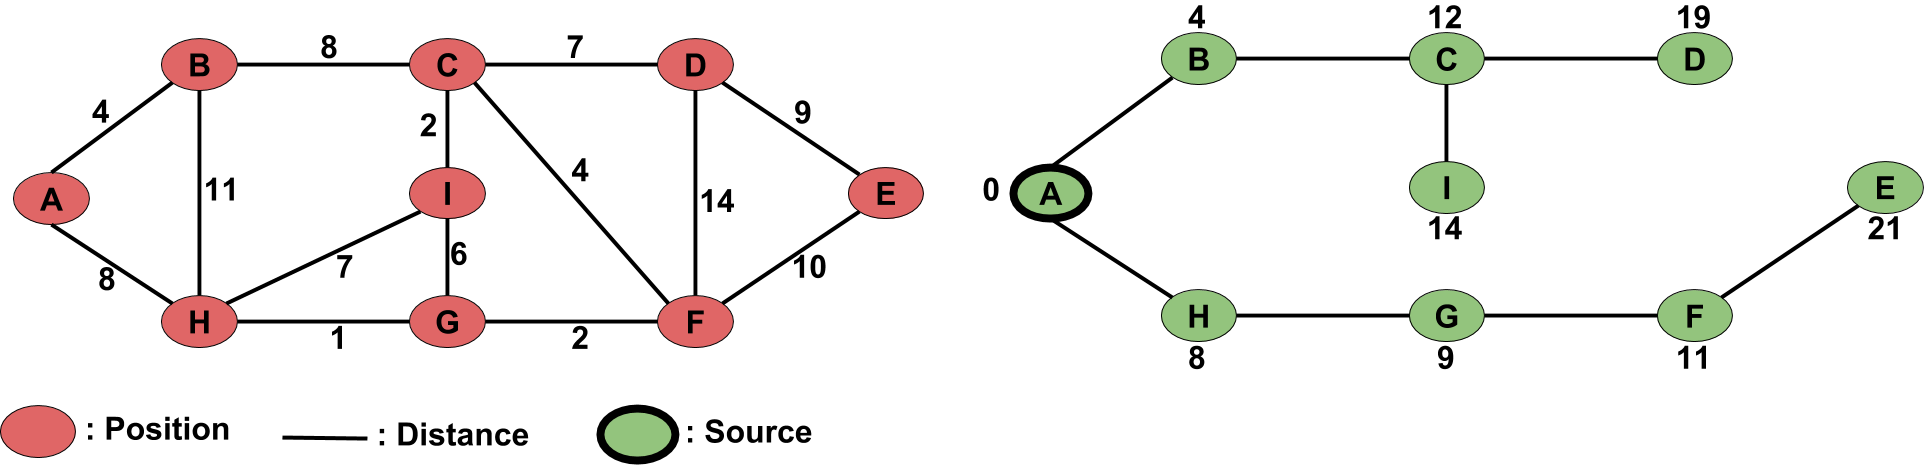
\includegraphics[width=160mm]{Figures/6.png}
\caption{Dijkstra pathfinding algorithm}
\end{center}
\end{figure*}
\vspace{-1cm}
\subsection{Detailed Routing}
The goal of detailed routing is to assign route segments of signal nets to specific routing tracks, vias, and metal layers with given global routes of those nets. For high performance analog circuits, constraints and objectives have to be considered. For the differential signal paths, the matching between parasitics on symmetrical nodes is often more important than their absolute values. For a given set of circuit specifications, several valid routing solutions can be found but with different yield, manufacturability and testability performances. Topology-matching and current-path constraints are commonly imposed on the critical, yet asymmetry nets with the same number of bends, vias, and wirelength to reduce current mismatches, sensitive nodes and noisy nodes that should not interact 

%----------------------------------------------------------------------------------------
%	THESIS CONTENT - APPENDICES
%----------------------------------------------------------------------------------------

\appendix % Cue to tell LaTeX that the following "chapters" are Appendices

% Include the appendices of the thesis as separate files from the Appendices folder
% Uncomment the lines as you write the Appendices

% Appendix A

\chapter{Frequently Asked Questions} % Main appendix title

\label{AppendixA} % For referencing this appendix elsewhere, use \ref{AppendixA}

\section{How do I change the colors of links?}

The color of links can be changed to your liking using:

{\small\verb!\hypersetup{urlcolor=red}!}, or

{\small\verb!\hypersetup{citecolor=green}!}, or

{\small\verb!\hypersetup{allcolor=blue}!}.

\noindent If you want to completely hide the links, you can use:

{\small\verb!\hypersetup{allcolors=.}!}, or even better: 

{\small\verb!\hypersetup{hidelinks}!}.

\noindent If you want to have obvious links in the PDF but not the printed text, use:

{\small\verb!\hypersetup{colorlinks=false}!}.

%\include{Appendices/AppendixB}
%\include{Appendices/AppendixC}

%----------------------------------------------------------------------------------------
%	BIBLIOGRAPHY
%----------------------------------------------------------------------------------------

\printbibliography



%----------------------------------------------------------------------------------------

\end{document}  
